%% BioMed_Central_Tex_Template_v1.06
%%                                      %
%  bmc_article.tex            ver: 1.06 %
%                                       %

%%IMPORTANT: do not delete the first line of this template
%%It must be present to enable the BMC Submission system to
%%recognise this template!!

%%%%%%%%%%%%%%%%%%%%%%%%%%%%%%%%%%%%%%%%%
%%                                     %%
%%  LaTeX template for BioMed Central  %%
%%     journal article submissions     %%
%%                                     %%
%%          <8 June 2012>              %%
%%                                     %%
%%                                     %%
%%%%%%%%%%%%%%%%%%%%%%%%%%%%%%%%%%%%%%%%%


%%%%%%%%%%%%%%%%%%%%%%%%%%%%%%%%%%%%%%%%%%%%%%%%%%%%%%%%%%%%%%%%%%%%%
%%                                                                 %%
%% For instructions on how to fill out this Tex template           %%
%% document please refer to Readme.html and the instructions for   %%
%% authors page on the biomed central website                      %%
%% http://www.biomedcentral.com/info/authors/                      %%
%%                                                                 %%
%% Please do not use \input{...} to include other tex files.       %%
%% Submit your LaTeX manuscript as one .tex document.              %%
%%                                                                 %%
%% All additional figures and files should be attached             %%
%% separately and not embedded in the \TeX\ document itself.       %%
%%                                                                 %%
%% BioMed Central currently use the MikTex distribution of         %%
%% TeX for Windows) of TeX and LaTeX.  This is available from      %%
%% http://www.miktex.org                                           %%
%%                                                                 %%
%%%%%%%%%%%%%%%%%%%%%%%%%%%%%%%%%%%%%%%%%%%%%%%%%%%%%%%%%%%%%%%%%%%%%

%%% additional documentclass options:
%  [doublespacing]
%  [linenumbers]   - put the line numbers on margins

%%% loading packages, author definitions

\documentclass[twocolumn]{bmcart}% uncomment this for twocolumn layout and comment line below
%\documentclass{bmcart}

%%% Load packages
%\usepackage{amsthm,amsmath}
%\RequirePackage{natbib}
%\RequirePackage[authoryear]{natbib}% uncomment this for author-year bibliography
%\RequirePackage{hyperref}
\usepackage[utf8]{inputenc} %unicode support
%\usepackage[applemac]{inputenc} %applemac support if unicode package fails
%\usepackage[latin1]{inputenc} %UNIX support if unicode package fails
\usepackage{amsmath, amsfonts, amssymb,amsthm, mathtools, thmtools, thm-restate, algorithm, algorithmicx, dsfont, cite, xcolor, xspace, multirow, caption}
\usepackage[bold]{complexity}
\usepackage[noend]{algpseudocode}

%%%%%%%%%%%%%%%%%%%%%%%%%%%%%%%%%%%%%%%%%%%%%%%%%
%%                                             %%
%%  If you wish to display your graphics for   %%
%%  your own use using includegraphic or       %%
%%  includegraphics, then comment out the      %%
%%  following two lines of code.               %%
%%  NB: These line *must* be included when     %%
%%  submitting to BMC.                         %%
%%  All figure files must be submitted as      %%
%%  separate graphics through the BMC          %%
%%  submission process, not included in the    %%
%%  submitted article.                         %%
%%                                             %%
%%%%%%%%%%%%%%%%%%%%%%%%%%%%%%%%%%%%%%%%%%%%%%%%%


%\def\includegraphic{}
%\def\includegraphics{}



%%% Put your definitions there:
\startlocaldefs
\newcommand{\note}[1]{(\textcolor{red}{#1})}
\newcommand{\opt}{\mathrm{OPT}}
\newcommand{\In}{\mathrm{In}}
\newcommand{\triv}{\mathrm{Triv}}
\newcommand{\ntriv}{\mathrm{NonTriv}}
\newcommand{\bs}{\mathrm{bisup}}
\newcommand{\RF}{\mathrm{RF}}
\newcommand{\bss}{\textsc{BSS}\xspace}
\newcommand{\rfs}{\textsc{RFS}\xspace}
\newcommand{\relaxed}{\textsc{Relax}-}
\newcommand{\bsstwo}{\textsc{BSS-$2$}\xspace}
\newcommand{\bssthree}{\textsc{BSS-$3$}\xspace}
\newcommand{\rftwo}{\textsc{RFS-$2$}\xspace}
\newcommand{\rfthree}{\textsc{RFS-$3$}\xspace}
\newcommand{\B}{\textsc{B}\xspace}
\renewcommand{\G}{\textsc{G}\xspace}
\renewcommand{\M}{\textsc{M}\xspace}
\DeclareMathOperator*{\argmin}{argmin}
\DeclareMathOperator*{\argmax}{argmax}
\DeclareMathOperator*{\extra}{Extra}
%\setlength\parindent{0pt}

\declaretheoremstyle[
spaceabove=10pt, spacebelow=10pt,
headfont=\normalfont\bfseries,
notefont=\mdseries, notebraces={(}{)},
bodyfont=\normalfont,
postheadspace=1em,
]{mystyle}
\theoremstyle{mystyle}
\newtheorem{theorem}{Theorem}
\newtheorem{lemma}{Lemma}
\newtheorem{claim}{Claim}
\newtheorem{corollary}{Corollary}
\newtheorem{definition}{Definition}

\declaretheoremstyle[
spaceabove=0pt, spacebelow=10pt,
headfont=\itshape,
notefont=\mdseries, notebraces={(}{)},
bodyfont=\normalfont,
postheadspace=1em,
headpunct = {:}
]{proofstyle}
\theoremstyle{proofstyle}
\newtheorem*{proof2}{Proof}
\newenvironment{proofnospace}{\begin{proof2}}{\qed \end{proof2}}

\captionsetup[table]{skip=10pt}

\endlocaldefs


%%% Begin ...
\begin{document}

\setlength{\abovedisplayskip}{6pt}
\setlength{\belowdisplayskip}{6pt}
\setlength{\abovedisplayshortskip}{3pt}
\setlength{\belowdisplayshortskip}{3pt}

%%% Start of article front matter
\begin{frontmatter}

\begin{fmbox}
\dochead{Research}

%%%%%%%%%%%%%%%%%%%%%%%%%%%%%%%%%%%%%%%%%%%%%%
%%                                          %%
%% Enter the title of your article here     %%
%%                                          %%
%%%%%%%%%%%%%%%%%%%%%%%%%%%%%%%%%%%%%%%%%%%%%%

\title{Solving the Robinson-Foulds Supertree Problem for Two Trees: Algorithms and Applications}

%%%%%%%%%%%%%%%%%%%%%%%%%%%%%%%%%%%%%%%%%%%%%%
%%                                          %%
%% Enter the authors here                   %%
%%                                          %%
%% Specify information, if available,       %%
%% in the form:                             %%
%%   <key>={<id1>,<id2>}                    %%
%%   <key>=                                 %%
%% Comment or delete the keys which are     %%
%% not used. Repeat \author command as much %%
%% as required.                             %%
%%                                          %%
%%%%%%%%%%%%%%%%%%%%%%%%%%%%%%%%%%%%%%%%%%%%%%

\author[
   addressref={UIUC},                   % id's of addresses, e.g. {aff1,aff2}
   %corref={aff1},                       % id of corresponding address, if any
   %noteref={n1},                        % id's of article notes, if any
   email={yuxilin51@gmail.com}   % email address
]{\inits{XY}\fnm{Xilin} \snm{Yu}}
\author[
   addressref={UIUC},
   email={thienle2@illinois.edu}
]{\inits{TL}\fnm{Thien} \snm{Le}}
\author[
   addressref={UIUC},
   email={sac@illinois.edu}
]{\inits{SC}\fnm{Sarah} \snm{Christensen}}
\author[
   addressref={UIUC},
   email={emolloy2@illinois.edu}
]{\inits{EKM}\fnm{Erin K.} \snm{Molloy}}
\author[
   addressref={UIUC},
   corref={UIUC},
   email={warnow@illinois.edu}
]{\inits{TW}\fnm{Tandy} \snm{Warnow}}

%%%%%%%%%%%%%%%%%%%%%%%%%%%%%%%%%%%%%%%%%%%%%%
%%                                          %%
%% Enter the authors' addresses here        %%
%%                                          %%
%% Repeat \address commands as much as      %%
%% required.                                %%
%%                                          %%
%%%%%%%%%%%%%%%%%%%%%%%%%%%%%%%%%%%%%%%%%%%%%%

\address[id=UIUC]{%                           % unique id
  \orgname{Department of Computer Science, University of Illinois at Urbana-Champaign}, % university, etc
  \street{201 N Goodwin},                     %
  \postcode{61820}                                % post or zip code
  \city{Urbana},                              % city
  \cny{US}                                    % country
}


%%%%%%%%%%%%%%%%%%%%%%%%%%%%%%%%%%%%%%%%%%%%%%
%%                                          %%
%% Enter short notes here                   %%
%%                                          %%
%% Short notes will be after addresses      %%
%% on first page.                           %%
%%                                          %%
%%%%%%%%%%%%%%%%%%%%%%%%%%%%%%%%%%%%%%%%%%%%%%

\begin{artnotes}
%\note{Sample of title note}     % note to the article
%\note[id=n1]{} % note, connected to author
\end{artnotes}

%\end{fmbox}% comment this for two column layout

%%%%%%%%%%%%%%%%%%%%%%%%%%%%%%%%%%%%%%%%%%%%%%
%%                                          %%
%% The Abstract begins here                 %%
%%                                          %%
%% Please refer to the Instructions for     %%
%% authors on http://www.biomedcentral.com  %%
%% and include the section headings         %%
%% accordingly for your article type.       %%
%%                                          %%
%%%%%%%%%%%%%%%%%%%%%%%%%%%%%%%%%%%%%%%%%%%%%%

\begin{abstractbox}

\begin{abstract} % abstract
\parttitle{Background} Supertree methods have been widely studied and used in phylogenetic tree estimation on large data sets as traditional tree estimation methods, such as maximum likelihood methods and Bayesian MCMC methods, are hard to scale. However, most current supertree methods do not have satisfying accuracy or scalability. A recent supertree method FastRFS, which solves a constrained version of the Robinson-Foulds Supertree problem (RFS) optimally, provides good accuracy and fast running time. However, the unconstrained RFS where the number of input trees is part of the input is \NP-hard and past attempts only provide heuristic methods. The complexity of RFS when there are only a constant number of input trees was unknown. 
\parttitle{Results} We present the first polynomial-time algorithm to solve the RFS problem on two input trees exactly, where the input trees do not need to binary. We also prove that RFS is \NP-hard when the input trees are general, even if there are only three input trees. These results not only cast light on major parts of the complexity landscape of RFS but also lead to a supertree method GreedyRFS that is comparable to its strong competitor FastRFS. GreedyRFS takes in a set of input trees and greedily chooses two trees to merge in each step using the algorithm for RFS on two trees. Experiments show that in tree error, GreedyRFS is very close to FastRFS with FastRFS having a slight advantage. In terms of criterion score, GreedyRFS performs slight better than FastRFS when the number of input trees is small and performs relatively close in general.
\parttitle{Conclusions}
BLAH-BLAH-BLAH
\end{abstract}

%%%%%%%%%%%%%%%%%%%%%%%%%%%%%%%%%%%%%%%%%%%%%%
%%                                          %%
%% The keywords begin here                  %%
%%                                          %%
%% Put each keyword in separate \kwd{}.     %%
%%                                          %%
%%%%%%%%%%%%%%%%%%%%%%%%%%%%%%%%%%%%%%%%%%%%%%

\begin{keyword}
Phylogeny, Robinson-Foulds Supertree, Polynomial-time Algorithm, NP-hardness, Greedy Algorithm
\end{keyword}

% MSC classifications codes, if any
%\begin{keyword}[class=AMS]
%\kwd[Primary ]{}
%\kwd{}
%\kwd[; secondary ]{}
%\end{keyword}

\end{abstractbox}
%
\end{fmbox}% uncomment this for twcolumn layout

\end{frontmatter}

%%%%%%%%%%%%%%%%%%%%%%%%%%%%%%%%%%%%%%%%%%%%%%
%%                                          %%
%% The Main Body begins here                %%
%%                                          %%
%% Please refer to the instructions for     %%
%% authors on:                              %%
%% http://www.biomedcentral.com/info/authors%%
%% and include the section headings         %%
%% accordingly for your article type.       %%
%%                                          %%
%% See the Results and Discussion section   %%
%% for details on how to create sub-sections%%
%%                                          %%
%% use \cite{...} to cite references        %%
%%  \cite{koon} and                         %%
%%  \cite{oreg,khar,zvai,xjon,schn,pond}    %%
%%  \nocite{smith,marg,hunn,advi,koha,mouse}%%
%%                                          %%
%%%%%%%%%%%%%%%%%%%%%%%%%%%%%%%%%%%%%%%%%%%%%%


%%%%%%%%%%%%%%%%%%%%%%%%%%%%%%%%%%%%%%%%%%%%%%%%%%%%%%%%%%%%%%%%%%%%%%%%%%%%%%%%%%%%%%%%%%%%%%%%
%%%%%%%%%%%%%%%%%%%%%%%%%%%%%%             Introduction            %%%%%%%%%%%%%%%%%%%%%%%%%%%%%
%%%%%%%%%%%%%%%%%%%%%%%%%%%%%%%%%%%%%%%%%%%%%%%%%%%%%%%%%%%%%%%%%%%%%%%%%%%%%%%%%%%%%%%%%%%%%%%%

\section{Introduction}
Phylogenetics is the study of evolutionary relationships between individuals and groups of organisms. Besides its immediate value of informing us about how the known species evolved on earth, it also helps us identify new species and predict how species may evolve in the future. Phylogeny estimation also enables researches to learn about origins of pathogens and thus develop either early detection methods or medicines for them \cite{phylogenymedicine}, to identify patterns of evolution of morphological and chemical characteristics \cite{phylogenycharacter}, and to develop ecological and biogeographical conservation strategies \cite{phylogenyconservation}.

With increasingly fast and cheap sequencing technologies, there has been an explosion of large-scale genomic data sets. This trend poses a continuing challenge to the algorithmic methods that researchers use to analyze genomic data and build phylogenetic trees. An increasingly important framework used on phylogeny estimation of large-scale data set is the divide-and-conquer framework. The first step of the framework is to decompose the sequence data into subsets of species so that a phylogenetic tree can be estimated on each subset individually and potentially in parallel. Then a supertree method is used to combine the trees on subsets of species into a tree of all species. The supertree estimation problem, which takes in a set of trees of different leaf sets that might be overlapping and builds a tree on the union of the leaf sets, was born out of the need to combine phylogenetic trees that have been previously estimated in different research projects to a larger tree and ultimately the Tree of Life. Besides the intended usage, supertree methods have also found their value in large-scale gene tree estimation and species tree estimation in the divide and conquer framework.   


\subsection{Related Work}
Most of the supertree methods attempt to approximately solve \NP-hard optimization problems with heuristics (e.g., Matrix Representation with Parsimony (MRP) \cite{MRP}\cite{MRPRagan}, Matrix Representation with Likelihood (MRL) \cite{MRL}, Mincut Supertree \cite{MinCut}, Quartets MaxCut \cite{QMaxCut}, Bad Clade Deletion \cite{BCD}). Among those \NP-hard optimization criteria, we focus on the  Robinson-Foulds (RF) distance, which measures the topological difference between two trees of the same leaf set. RF distance is an extensively used metric to evaluate the accuracy of supertree estimation methods either with respect to the true model tree or with respect to the input trees. As such, it is expected that solving the Robinson-Foulds Supertree (RFS) problem, which directly minimizes the RF distance between the supertree and the input trees, can lead to highly accurate results. Other than the obvious benefit, RFS is also shown to be closely related to the Maximum Likelihood Supertree problem under the exponential error model studied in \cite{MLS}.
However, it is shown that RFS is \NP-hard for arbitrary number of input trees, even when all input trees are binary \cite{RFScomplexity}.

The RFS problem was first considered in the phylogenetic setting in \cite{RFS}, where a heuristic method for the special case of rooted input trees was proposed. Later, the heuristic method was generalized to both rooted and unrooted input trees \cite{RFSunrooted}. 
%Xilin - add more references to papers with methods for RFS. Get them from the FastRFS paper.
The recently developed method FastRFS, instead of offering another heuristic, solves a constrained version of RFS exactly and is proven to be both accurate and fast \cite{FastRFS}. 

The RFS problem is equivalent to the less known Bipartition Support Supertree (BSS) problem, which finds a binary supertree that maximizes the number of bipartitions shared by the supertree and the input trees. 
%Xilin, if this wasn't proven anywhere, it's worth restating this a bit; otherwise, add a reference.
However, when the output tree is relaxed to not necessarily be binary, 
\textcolor{blue}{we will show that }
the BSS problem is different from the RFS problem
\textcolor{blue}{(Theorem XX)}, 
and can be of independent interests. 
Requiring a supertree to be binary may artificially introduce edges that are not well supported by the input trees and thus it might be desirable to allow the output tree to be non-binary. 

\subsection{Results}
Even though the RFS problem is \NP-hard on arbitrary number of input trees, the complexity of the problem on a small constant number (e.g., two or three) of input trees was not known. Also, past studies have also mostly assumed that input trees are binary, which limits the scope of the problem. 

We show that RFS can be solved exactly in polynomial time when there are only two input trees 
\textcolor{blue}{(Theorem XX)},
and this result applies to the general case (i.e., for arbitrary input trees).
We also show that RFS is NP-hard when input trees are general, even if there are only three input trees 
\textcolor{blue}{(Theorem XX)}. 
Both of our algorithmic and hardness results for RFS derive from the equivalence of RFS to BSS and the algorithmic and hardness results for the BSS problem, which we establish in \textcolor{blue}{(Theorem XX)}. 
The algorithmic and hardness results for BSS can be easily adapted for the relaxed version of the problem where the output is not necessarily binary, but the relaxed version of BSS is not equivalent to a relaxed version of RFS 
\textcolor{blue}{(Theorem XX)}, and these result do not transfer to a relaxed version of RFS. We summarize our theoretical results in Table \ref{tab:complexity_summary}.

\renewcommand{\arraystretch}{1.5}
\begin{table}[t]
    \centering
    % \begin{tabular}{|c|c|c|c|c|c|}
    %     \hline
    %       \multicolumn{6}{|c|}{Input Trees}\\
    %     \hline
    %      \multicolumn{3}{|c|}{Binary}  & \multicolumn{3}{|c|}{General}\\
    %     \hline
    %      $2$ & $3$ & $N$ & $2$ & $3$ & $N$\\
    %     \hline
    %      \P($\star$) & ? & \NP-hard \cite{RFScomplexity} & \P($\star$) & \multicolumn{2}{|c|}{\NP-hard($\star$)}\\
    %     \hline
    % \end{tabular}
        \begin{tabular}{|c|c|c|c|c|c|c|}
        \hline
          \multirow{3}{4em}{Problem} & \multicolumn{6}{|c|}{Input Trees}\\
        \cline{2-7}
         &\multicolumn{3}{|c|}{Binary}  & \multicolumn{3}{|c|}{General}\\
        \cline{2-7}
         &$2$ & $3$ & $N$ & $2$ & $3$ & $N$\\
        \hline
         RFS / BSS & \P($\star$) & ? & \NP-hard \cite{RFScomplexity} & \P($\star$) & \multicolumn{2}{|c|}{\NP-hard($\star$)}\\
        \hline
         Relaxed BSS & \P($\star$) & \multicolumn{2}{|c|}{?} & \P($\star$) & \multicolumn{2}{|c|}{\NP-hard($\star$)}\\
        \hline
    \end{tabular}
    \caption[Summary of complexity of RFS]{Summary of complexity of RFS (RFS) and BSS. In the table, the results with ($\star$) are new from this paper and the question marks show open questions. We show the algorithmic results in Theorem \ref{thm:correctness_alg} and Corollary \ref{cor:correctness_alg} and proof the hardness results in Theorem \ref{thm:hardness}.}
    \label{tab:complexity_summary}
\end{table}

We incorporate the algorithm for RFS on two input trees into a greedy algorithm, GreedyRFS, that computes a supertree for arbitrary number of input trees. The greedy algorithm chooses two trees whose intersection of leaf set has the maximum cardinality among all pairs of trees and use the exact algorithm to merge these two trees. With the merged supertree added back to the list of trees to be merged, the greedy algorithm repeatedly merge two trees from the list until one supertree remains. 

\note{more on experiments results later}

%%%%%%%%%%%%%%%%%%%%%%%%%%%%%%%%%%%%%%%%%%%%%%%%%%%%%%%%%%%%%%%%%%%%%%%%%%%%%%%%%%%%%%%%%%%%%%%%
%%%%%%%%%%%%%%%%%%%%%%%%%%%%%%             Preliminary             %%%%%%%%%%%%%%%%%%%%%%%%%%%%%
%%%%%%%%%%%%%%%%%%%%%%%%%%%%%%%%%%%%%%%%%%%%%%%%%%%%%%%%%%%%%%%%%%%%%%%%%%%%%%%%%%%%%%%%%%%%%%%%


\section{Terminologies and Problem Statements}\label{sec:prelim}
In this section, we introduce basic terminologies and formal problem statements. 

Throughout the paper, we consider only unrooted leaf-labelled trees, but we do not constrain them to be binary. For any tree $T$, let $V(T)$, $E(T)$, $L(T)$, $\In(T)$ denote the vertices, edges, leaves, and internal nodes of $T$, respectively. Let $\mathcal{T}_S$ denote the set of all trees such that $L(T) = S$. For any $v\in V(T)$, let $N_T(v)$ denote the set of neighbors of $v$ in $T$. 

In any tree $T$, each edge $e$ induces a bipartition $\pi_e := A|B$ of the leaf set, where $A$ and $B$ are the leaves in the two components of $T-e$. A bipartition $A|B$ is non-trivial if both sides have size at least $2$. For a tree $T$, $C(T) := \{\pi_e \mid e\in E(T)\}$ denotes the set of all bipartitions of $T$. A tree $T'$ is a \textit{refinement} of $T$ if $T$ can be obtained from $T'$ by contracting a set of edges. Equivalently, $T'$ is a refinement of $T$ if and only if $C(T) \subseteq C(T')$. A tree is \textit{fully resolved} or \textit{binary} if every non-leaf node has degree $3$. (We will use fully resolved and binary interchangeably.) Equivalently, a tree $T$ with $n$ leaves is fully resolved if and only if $C(T)$ contains $2n-3$ bipartitions, exactly $n-3$ of which are non-trivial. A tree $T$ is \textit{minimally resolved} with respect to a tree score if no $e \in E(T)$ can be contracted without changing the score of $T$. 

Two bipartitions $\pi_1$ and $\pi_2$ of the same leaf set are \textit{compatible} if and only if there exists a tree $T$ such that $\pi_1, \pi_2 \in C(T)$. A tree $T$ restricted to a subset $R$ of its leaf set, denoted $T|_R$, is the minimal subtree of $T$ spanning $R$ with nodes of degree two suppressed. A bipartition $\pi = A|B$ restricted to a subset $R \subseteq A\cup B$ is $\pi|_R = A\cap R | B\cap R$. For any positive integer $n$, let $[n]$ denote $\{1,2,\dots,n\}$. For any set $S$ and element $a$, $S-a:= S\backslash \{a\}$. For any graph $G$ and $v \in V(G)$, $(u,w)\in E(G)$, we also use $G - v$ or $G -(u,w)$ to represent the graph obtained from deleting $v$ from $G$ or deleting $(u,w)$ from $G$, separately.


We have the following definition of Robinson-Foulds distance \cite{RF} and bipartition support where the former measures differences between the topology of the trees and the latter measures the similarity.
\begin{definition}
For two trees $T$, $T'$ with the same leaf set, the \textit{Robinson-Foulds distance} of them is $\RF(T, T') := |C(T)\backslash C(T')| + |C(T') \backslash C(T)|$.
\end{definition}

\begin{definition}
For two trees $T$, $T'$ with the same leaf set, the \textit{bipartition support} of them is $\bs(T, T') := |C(T) \cap C(T')|$.
\end{definition}

%Xilin, you need to cite at least one reference to Robinson-Foulds Supertrees. But also, I don't like the definition of the RFS problem as follows, since it seems to follow the definition of X and seems to require that the input have a certain form. Please rework this so that the RFS problem is defined without giving the impression that all pairs of trees in the input have the same pairwise intersection.

Let $T_1,T_2,\dots,T_N$ be a set of $N$ trees with leaf sets $S_1,S_2,\dots,S_N$, respectively. Let $S := \bigcup_{i \in [N]}S_i$. 
The Robinson-Foulds supertree problem \cite{RFS} on these $N$ trees, abbreviated \rfs, finds a fully resolved supertree $T^* \in \mathcal{T}_S$ such that
\[T^* = \argmin_{T \in \mathcal{T}_S} \sum_{i \in [N]} \RF(T|_{S_i}, T_i).\]

The maximum bipartition support supertree problem on these $N$ trees, abbreviated \bss, finds a fully resolved supertree $T^* \in \mathcal{T}_S$ such that
\[T^* = \argmax_{T \in \mathcal{T}_S} \sum_{i \in [N]} \bs(T|_{S_i}, T_i).\]

We will later show (\textcolor{blue}{Theorem XX}) that these two problems are equivalent. For both \rfs and \bss, we can relax the requirement of the output to allow the output to be non-binary, and we denote the relaxed version of the \rfs and \bss problems by \relaxed\rfs and \relaxed\bss, respectively. 

We call $\sum_{i \in [N]} \RF(T|_{S_i}, T_i)$ the RF score of $T$ when $T_i$'s are clear from context. Similarly, the support score of $T$ is $\sum_{i\in[N]}\bs(T|_{S_i}, T_i)$. 

We pay attention to the special case of the problems where there are only two or three input trees and we specify the number in the problem name. 
We also introduce different variants of \rfs and \bss with the input trees being either binary (B) or general (G), and we append this to the problem name. For example, the RFS problem with two binary input trees is \rftwo-\B, the relaxed BSS problem with three general input trees and a general output supertree is \relaxed\bssthree-\G. 

We note \bss or \rfs with binary output tree is a different optimization problem than \relaxed\bss or \relaxed\rfs with general output tree; however, we will show that
when the output tree has the same requirement, 
\bss-\B or \rfs-\B with binary input trees is a special case of \bss-\G or \rfs-\G with general input trees. 

%%%%%%%%%%%%%%%%%%%%%%%%%%%%%%%%%%%%%%%%%%%%%%%%%%%%%%%%%%%%%%%%%%%%%%%%%%%%%%%%%%%%%%%%%%%%%%%%
%%%%%%%%%%%%%%%%%%%%%%%%%%%%%%           Theory Result             %%%%%%%%%%%%%%%%%%%%%%%%%%%%%
%%%%%%%%%%%%%%%%%%%%%%%%%%%%%%%%%%%%%%%%%%%%%%%%%%%%%%%%%%%%%%%%%%%%%%%%%%%%%%%%%%%%%%%%%%%%%%%%

\section{Theoretical Results} \label{sec:theory}

In this section, we present our theoretical results. For brevity, we only give a proof sketch for most of the lemmas and include the full proofs in the appendix.  

First, we present out main result. Let $T_1,T_2,S_1$, and $S_2$ be defined as from the problem statement for \rftwo. Let Let $X:= S_1 \cap S_2$.
%Xilin, you had the same label for both theorems, so I gave them separate numbers
\begin{restatable}{theorem}{thmCorrectAlg_1} \label{thm:correctness_alg}
%Xilin, this is not grammatical (you had "both"), so I removed "both" here and in a theorem below
   % Both 
    \rftwo-\G can be solved in $O(n^2|X|)$ time, where $n :=\max\{|S_1|,|S_2|\}$.
\end{restatable}
This theorem relies on the equivalence of corresponding variants of \rfs and \bss and on the following theorem for \bsstwo.
    
\begin{restatable}{theorem}{thmCorrectAlg_2}
    \bsstwo-\G and \relaxed\rftwo-\G can be solved in $O(n^2|X|)$ time, where $n :=\max\{|S_1|,|S_2|\}$.
\end{restatable}    
  
  %Xilin, this is not grammatical (you had "both"), so I removed "both"  
\begin{corollary}\label{cor:correctness_alg}
   % Both 
    \rftwo-\B can be solved in $O(n^2|X|)$ time, where $n :=\max\{|S_1|,|S_2|\}$.
\end{corollary}
This corollary follows trivially from Theorem \ref{thm:correctness_alg} as \rftwo-\B-\B and \rftwo-\B-\G are special cases of \rftwo-\G-\B and \rftwo-\G-\G, separately. To prove Theorem \ref{thm:correctness_alg}, we first present Algorithm \ref{alg:maxbisup} which solves \bsstwo-\G-\M in $O(n^2|X|)$ time. Then we will prove the equivalence between \bsstwo-\G-\M and \rftwo-\G-\G and the equivalence between \bsstwo-\G-\B and \rftwo-\G-\B. We will also briefly talk about how Algorithm \ref{alg:maxbisup} with one extra step can solve \bsstwo-\G-\B in the same asymptotic time. 

We begin with some additional terminology
and notation. 
In the following part, we use $i\in[2]$ to index the two input trees. 
\textcolor{blue}{
We will refer to $T_i|_X$ as the backbone tree of $T_i$. }
Let $\Pi$ be the set of bipartitions of $X$. Let $\triv$ and $\ntriv$ denote the set of trivial and non-trivial bipartitions in $C(T_1|_X) \cup C(T_2|_X)$.
For $R\subseteq L(T)$ and $e \in E(T|_R)$, let $P_T(e)$ denote the path in $T$ from which $e$ is obtained by suppressing degree-two nodes, and we denote $P_T(e)$ by $P(e)$ when $T$ is clear from context.
For any $e \in E(T_i|_X)$, let $w(e):= |P_{T_i}(e)|$, i.e., $w(e)$ is the number of edges on the path in $T_i$ from which $e$ is obtained by suppressing degree two nodes. 
For any bipartition $\pi$ of $X$, let $e_i(\pi)$ denote the edge that induces $\pi$ in $T_i|_X$. We define a weight function $w:\Pi \to \mathbb{N}_{\ge 0}$ such that for any bipartition $\pi$ of $X$, $w(\pi) = w(e_1(\pi)) + w(e_2(\pi))$. If $e_i(\pi)$ does not exist, we use $w(e_i(\pi)) = 0$. Therefore, for any $\pi \notin C(T_1|_X) \cup C(T_2|_X)$, $w(\pi) = 0$. For any set $F$ of bipartitions, $w(F) = \sum_{\pi \in F} w(\pi)$. 

For each $e \in E(T_i|_X)$, let $\In(e)$ be the set of internal nodes of $P_{T_i}(e)$. We note that $|\In(e)| = w(e)-1$. For any $v \in \In(T_i|_X)$ or any $v \in \In(e)$ for some $e \in E(T_i|_X)$, let $L(v)$ be the set of leaves in $S_i \backslash X$ whose connecting path to $T_i|_X$ goes through $v$ and let $\mathcal{T}(v)$ be the set of subtrees containing vertices of $L(v)$ in $T_i - v$. We say $\mathcal{T}(v)$ is a set of extra subtrees attached to $v$. Consider each subtree in $\mathcal{T}(v)$ rooted at the node $u$ which is a neighbor of $v$. Let $\mathcal{T}(e) := \bigcup_{v \in \In(e)} \mathcal{T}(v)$ be the set of extra subtrees attached to $e$. For any bipartition $\pi = A|B \in C(T_1|_X) \cup C(T_2|_X)$, we denote $\mathcal{T}(\pi) := \bigcup_{i \in [2]} \mathcal{T}(e_i(\pi))$. Let $C_i(A), C_i(B)$ be the components in $T_i|_X - e_i(\pi)$ containing $A$ and $B$, separately. For $Q = A$ or $B$, let $\mathcal{T}_i(Q) = \bigcup_{e \in E(C_i(Q))} \mathcal{T}(e) \cup \bigcup_{v \in In(C_i(Q))} \mathcal{T}(v)$. Then $\mathcal{T}_i(Q)$ denotes the set of extra subtrees in $T_i$ on the side of $Q$, i.e., in $C_i(Q)$. Let $\extra(T_i) := \bigcup_{e \in E(T_i|_X)} \mathcal{T}(e) + \bigcup_{v \in \In(T_i|_X)} \mathcal{T}(v)$ be the set of extra subtrees in $T_i$. We note that by definition $\extra(T_i) = \mathcal{T}_i(A) + \mathcal{T}_i(B) + \mathcal{T}(e_i(\pi))$ for any $\pi \in \Pi$. Let $\extra := \extra(T_1) \cup \extra(T_2)$ denote the set of all extra subtrees in $T_1$ and $T_2$.  

\begin{figure}
    \centering
    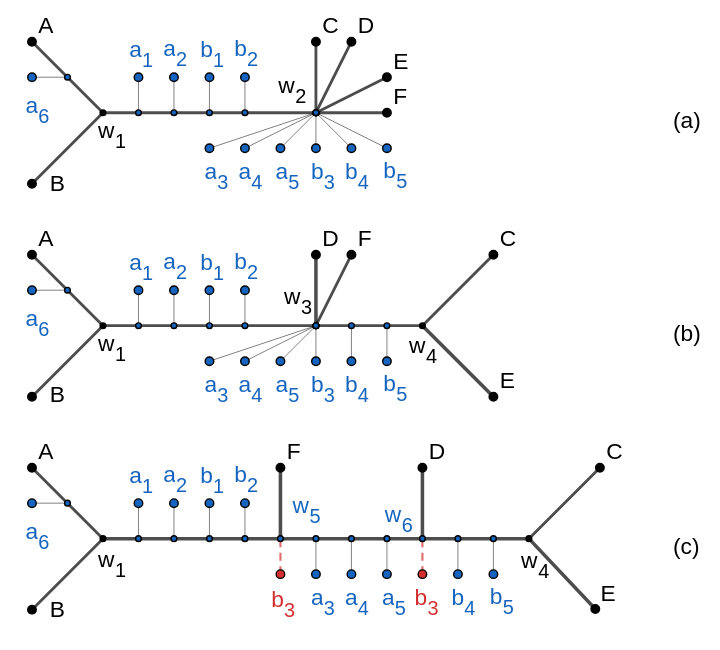
\includegraphics[scale = 0.75]{refinement_procedure.png}
    \caption{Caption}
    \label{fig:my_label}
\end{figure}

Let $G = (V=V_1 \cup V_2, E)$ be the incompatibility graph on $C(T_1|_X) \cup C(T_2|_X)$, such that $V_1 = C(T_1|_X)$ and $V_2 = C(T_2|_X)$, and $E = \{(\pi, \pi') \mid \pi \in V_1, \pi' \in V_2$, $\pi$ is not compatible with $\pi'\}$. We note that $G$ is a bipartite graph since for both $i=1,2$, $C(T_i|_X)$ is a compatible set and thus $V_i$ is independent. 

We differentiate between two kinds of bipartitions in $\mathcal{C}=C(T_1) \cup C(T_2)$. Let 

$$\Pi_Y = \{ A|B \in \mathcal{C} \mid \text{either } A\cap X = \emptyset \text{, or } B \cap X = \emptyset\}$$  and 
$$\Pi_X = \{ A|B \in \mathcal{C} \mid A\cap X \neq \emptyset \text{ and } B\cap X \neq \emptyset \}.$$

Intuitively, $\Pi_X$ is the set of bipartitions in  $\mathcal{C}$ that are induced by edges in the minimal subtree spanning $X$, and $\Pi_Y$ is the set of bipartitions in  $\mathcal{C}$ induced by edges not in the minimal subtree spanning $X$, i.e., induced by edges inside extra subtrees or connecting extra subtrees to the backbone trees. 

Let $p_X(\cdot)$ and $p_Y(\cdot)$ be scores on trees of leaf set $S$ such that
\begin{align*}
    p_X(T) &= \sum_{i \in [2]}|C(T|_{S_i}) \cap C(T_i) \cap \Pi_X|,\\
    p_Y(T) &= \sum_{i \in [2]} |C(T|_{S_i}) \cap C(T_i) \cap \Pi_Y|.
\end{align*}


Intuitively, $p_X(T)$ and $p_Y(T)$ decomposes the support score of $T$ into the score contributed by bipartitions in $\Pi_X$ and the score contributed by bipartitions in $\Pi_Y$ and the two scores can be maximized sequentially without interference. 

This is exactly what Algorithm \ref{alg:maxbisup} does in three stages. It first construct a tree $T$ that maximizes the $p_Y(\cdot)$ score. Then it builds an incompatibility graph $G$ on $C(T_1|_X) \cup C(T_2|_X)$ and finds a maximum weight independent set $I$ of $G$ that represents a set of compatible bipartitions of $C(T_1|_X) \cup C(T_2|_X)$ whose addition to $T|_X$ gives the maximum potential $p_X(\cdot)$ score. In the end, the algorithm refines $T$ by adding each $\pi \in I$ to $T|_X$ through Algorithm \ref{alg:refine} to realize the maximum potential $p_X(\cdot)$ score for $T$. We note that the order in which the algorithm adds the bipartitions in $I$ does not matter, but for technical reasons, the algorithm actually adds all trivial bipartitions first and then the non-trivial ones.


\begin{algorithm}
    \caption{Max-BiSup Supertree}%
    \label{alg:maxbisup}
    \begin{algorithmic}[1]
        \Statex \textbf{Input}: two input trees $T_1$, $T_2$ with leaf sets $S_1$ and $S_2$ where $S_1 \cap S_2 = X \neq \emptyset$ 
        \Statex \textbf{Output}: a supertree $T$ on leaf set $S = S_1 \cup S_2$ that maximizes the support score
        \State compute $C(T_1|_X)$ and $C(T_2|_X)$
        \For{each $\pi \in C(T_1|_X) \cup C(T_2|_X)$}
            \For{$i \in [2]$}
                \State compute $\mathcal{T}(e_i(\pi))$, $\mathcal{T}_i(A)$ and $\mathcal{T}_i(B)$
            \EndFor
            \State compute $\mathcal{T}(\pi)$ and $w(\pi)$
        \EndFor
        \State construct $T$ as a star of leaf set $X$ with center vertex $\hat{v}$ with the root of each $t \in \extra$ connected to $\hat{v}$  \Comment{let $\hat{T} = T$}       
        \For{each $\pi = \{a\}|B \in \triv$}
            %\State $T \gets $ Refine-Triv($T_1, T_2, T, \pi, \hat{v}, \mathcal{T}$) \Comment{let $\tilde{T} = T$ after for loop}
            \State detach all extra subtrees in $\mathcal{T}(\pi)$ from $\hat{v}$ and attach them onto $(\hat{v},a)$ such that the subtrees from $\mathcal{T}(e_1(\pi))$ and subtrees from $\mathcal{T}(e_2(\pi))$ are side by side and the attachments of $\mathcal{T}(e_i(\pi))$ matches the their attachment on $e_i(\pi)$ exactly
        \EndFor \Comment{let $\tilde{T} = T$ after for loop}
        \State construct the incompatibility graph $G$ of $T_1|_X$ and $T_2|_X$ 
        \State compute the maximum weight independent set $I'$ in $G - (C(T_1|_X) \cap C(T_2|_X)$ with weight $w$
        \State let $I = I' \cup (C(T_1|_X) \cap C(T_2|_X))$, let $H(\hat{v}) = \ntriv $, let $sv(\pi) = \hat{v}$ for all $\pi \in \ntriv$
        \For{each $\pi \in \ntriv \cap I$}
            \State $T \gets $ Refine($T_1,T_2, T, \pi, H, sv, \mathcal{T}$) 
        \EndFor \Comment{let $T^* = T$ after for loop}
        \State return $T$
    \end{algorithmic}
\end{algorithm}

The refinement phase, i.e., Algorithm \ref{alg:refine}, works in five steps. In the first step (lines $1-2$), it obtains the vertex $v$ to split for adding the new bipartition $\pi$ from the data structure $sv$ and splits $v$ into $v_a$ and $v_b$. In the second step (lines $3-6$), it divides the neighbors of $v$ in $T|_X$ appropriately and connects the ones which can reach $A$ to $v_a$ and the ones which can reach $B$ to $v_b$. In the third step (line $7$), it moves all extra subtrees in $\mathcal{T}(\pi)$ onto the new edge $(v_a,v_b)$ in a particular way to make sure the $w(\pi)$ partitions from $T_1$ and $T_2$ which become $\pi$ when restricted to $X$ are all included in $T|_{S_1}$ or $T|_{S_2}$. 
Next, it moves other extra subtrees which should be in the same component as $A$ (or $B)$ in $T_i - e_i(\pi)$, i.e., those in $\mathcal{T}_i(A)$ (or $\mathcal{T}_i(B)$), to the side of $v_a$ (or $v_b$). 
\textcolor{blue}{
It also moves the remaining extra subtrees either $v_a$ or $v_b$ because they do not matter. }
%Xilin, I think you are missing "to" in this sentence above. ALso, for the next sentence, I don't think H(v_a) has been defined.
In the last step, it updates the auxiliary data structures such 
\textcolor{blue}{
that $H(v_a)$ or $H(v_b)$} now contains the bipartitions that can be added by a refinement at $v_a$ or $v_b$, respectively, and for each bipartition $\pi$, $sv(\pi)$ is the vertex to split to add $\pi$.

\begin{algorithm}
    \caption{Refine}
    \label{alg:refine}
    \begin{algorithmic}[1]
        \Statex \textbf{Input}: two trees $T_1$, $T_2$ with leaf sets $S_1$ and $S_2$ where $S_1 \cap S_2 = X \neq \emptyset$, an unrooted tree $T$ on leaf set $S = S_1 \cup S_2$, a nontrivial bipartition $\pi = A|B$ of $X$, a dictionary $H$, a dictionary $sv$, a dictionary $\mathcal{T}$
        \Statex \textbf{Output}: an tree $T'$ which is a refinement of $T$ such that $C(T|_X) \backslash C(T'|_X) = \{\pi\}$ 
        \State $v \gets sv(\pi)$
        \State $V(T) \gets V(T) \cup \{v_a, v_b\}$, $E(T) \gets E(T) \cup \{(v_a,v_b)\}$
        \State compute $N_A:= \{u \in N_{T|_X}(v) \mid $ there $\exists a \in A$ such that $u$ can reach $a$ in $T|_X-v \}$ and $N_B:= \{u \in N_{T|_X}(v) \mid$ there $\exists b \in B$ such that $u$ can reach $b$ in $T|_X-v\}$. 
        \For{each $u \in N_A \cup N_B$} 
            \If{$u \in N_A$} connect $u$ to $v_a$
            \Else{} connect $u$ to $v_b$
            \EndIf
        \EndFor
        \State detach all extra subtrees in $\mathcal{T}(\pi)$ from $v$ and attach them onto $(v_a,v_b)$ such that the subtrees from $\mathcal{T}(e_1(\pi))$ and subtrees from $\mathcal{T}(e_2(\pi))$ are side by side and the attachments of $\mathcal{T}(e_i(\pi))$ matches their attachment on $e_i(\pi)$ exactly
        \For{each $t \in \mathcal{T}_1(A) \cup \mathcal{T}_2(A)$ that is attached to $v$}
            \State detach $t$ from $v$ and attach it to $v_a$
        \EndFor
        \For{each $t \in \mathcal{T}_1(B) \cup \mathcal{T}_2(B)$ that is attached to $v$}
            \State detach $t$ from $v$ attach $t$ to $v_b$
        \EndFor
        \For{each remaining extra subtree attached to $v$}
            \State detach it from $v$ and attach it to either $v_a$ or $v_b$
        \EndFor
        \State $H(v_a) \gets \emptyset, H(v_b) \gets \emptyset$
        \For{each bipartition $\pi'= A'|B' \in H(v)$ such that $\pi' \neq \pi$}
            \If{$A' \subseteq A$ or $B' \subseteq A$}
                \State $sv(\pi') = v_a$, $H(v_a) \gets H(v_a) + \pi'$
            \ElsIf{$A' \subseteq B$ or $B' \subseteq B$}
                \State $sv(\pi') = v_b$, $H(v_b) \gets H(v_b) + \pi'$
            \Else{} 
                \State discard $\pi'$
            \EndIf
        \EndFor
        \State delete $v$ and incident edges from $T$ and return the resulting tree $T'$
    \end{algorithmic}
\end{algorithm}
 

\begin{restatable}{lemma}{lemMaxPY}\label{lem:max_pY}
    For any tree $T$ of leaf set $S$, $p_Y(T) \le |\Pi_Y|$. In particular, let $\hat{T}$ be the tree defined in Algorithm \ref{alg:maxbisup}. Then, $p_Y(\hat{T}) = |\Pi_Y|$. 
\end{restatable}
Lemma \ref{lem:max_pY} formally states that the tree $\hat{T}$ we build at the beginning of the algorithm maximizes the $p_Y(\cdot)$ score. Intuitively, this lemma is true because there are only $|\Pi_Y|$ bipartitions that can contribute to $p_Y(\cdot)$. Each of these bipartitions is either induced by an edge in an extra subtree or induced by an edge connecting an extra subtree to the backbone tree and $\hat{T}$ contains all of them by construction.  

\begin{restatable}{lemma}{lemOneBiparUpperbound} \label{lem:one_bipar_upperbound}
    Let $\pi = A|B \in \Pi$. Let $T$ be a tree of leaf set $S$ such that $\pi \notin C(T|_X)$ and all bipartitions in $C(T|_X)$ are compatible with $\pi$. Let $T'$ be a refinement of $T$ such that for all $\pi' \in C(T'|_{S_i}) \backslash C(T|_{S_i})$ for some $i \in [2]$, $\pi'|_X = \pi$. Then, $p_X(T') - p_X(T) \le w(\pi)$. 
\end{restatable}

\begin{restatable}{lemma}{lemCompatibleSetUpperbound} \label{lem:compatible_set_upperbound}
    For any compatible set $F$ of bipartitions in $\Pi$, let $T$ be a tree of leaf set $S$ such that $C(T|_X) = F$. Then $p_X(T) \le \sum_{\pi \in F} w(\pi)$.
\end{restatable}
Lemma \ref{lem:one_bipar_upperbound} shows that the weight function we define on each bipartition of $X$ represents the maximum potential increase in $p_X(\cdot)$ as a result of adding that bipartition to $T|_X$. The proof of Lemma \ref{lem:one_bipar_upperbound} follows the idea that for any bipartition $\pi$ of $X$, there are at most $w(\pi)$ edges in either $T_1$ or $T_2$ whose induced bipartition becomes $\pi$ when it is restricted to $X$. Therefore, by only adding $\pi$ to $T|_X$, there are at most $w(\pi)$ more bipartitions in $C(T|_{S_1})$ or $C(T|_{S_2})$ that contributes to the increase of $p_X(T)$. The proof of Lemma \ref{lem:compatible_set_upperbound} uses Lemma \ref{lem:one_bipar_upperbound} repeatedly by adding the compatible bipartitions to the tree in an arbitrary order. 

\begin{restatable}{claim}{claimAfterAddTrivial}\label{claim:after_add_trivial}
    Let $\tilde{T}$ be the tree constructed in Algorithm \ref{alg:maxbisup}, then $p_X(\tilde{T}) = \sum_{\pi \in \triv} w(\pi)$. 
\end{restatable}
The above claim states that the algorithm adds the trivial bipartitions of $X$ to $T|_X$ in a way such that $p_X(T)$ actually reaches the full potential of adding each of those trivial bipartitions. The proof naturally follows from the way we attach extra subtrees in Line $8$ of Algorithm \ref{alg:maxbisup}.  

 
\begin{restatable}{lemma}{lemRefineAchievesWeight} \label{lem:refine_achieves_weight}
Let $T$ be a tree from Algorithm \ref{alg:maxbisup} before a refinement step. Let $\pi = A|B \in \ntriv \cap I$. Let $T'$ be a refinement of $T$ obtained from running Algorithm \ref{alg:refine} on $T$ and $\pi$, with the auxiliary data structures $H$, $sv$, and $\mathcal{T}$. Then, $p_X(T') - p_X(T) = w(\pi)$. 
\end{restatable}
Lemma \ref{lem:refine_achieves_weight} shows that Algorithm \ref{alg:refine} adds any non-trivial bipartition of $X$ to the $T|_X$ in a way that realizes the maximum potential increase of $p_X(T)$ of adding that bipartition. The proof mainly relies on three invariants of Algorithm \ref{alg:refine}. One is that the auxiliary data structures $H$ and $sv$ makes sure that we can correctly find the vertex to split to add any bipartition to $T|_X$. Second is that the extra subtrees of any bipartition $\pi$ to be added are attached to the splitting vertex $sv(\pi)$. Third is that we always make sure that for any bipartition in $C(T|_X)$, the extra subtrees in $\mathcal{T}_i(A)$ or $\mathcal{T}_i(B)$ are attached to the right side of the tree. With these invariants, for any bipartition $\pi$ to be added, Algorithm \ref{alg:refine} is able to split the vertex correctly and move extra subtrees around in a way such that each bipartition in $T_1$ or $T_2$ that is induced by an edge in $P(e_1(\pi))$ or in $P(e_2(\pi))$ is present in $T_|{S_1}$ or $T_|{S_2}$ after the refinement. There are exactly $w(\pi)$ such bipartitions and they contribute $w(\pi)$ to $p_X(T)$. 


\begin{restatable}{claim}{claimMaxCompatibleSubset} \label{claim:max_compatible_subset}
    Let $I$ be defined as in Algorithm \ref{alg:maxbisup}. $I$ is a maximum weight compatible subset of $C(T_1|_X) \cup C(T_2|_X)$. 
\end{restatable}
This claim follows naturally from the fact that $I$ is a maximum weight independent set in the incompatibility graph $G$ where any two bipartitions in $C(T_1|_X) \cup C(T_2|_X)$ have an edge between them if and only if they are incompatible.

\begin{restatable}{lemma}{lemEquivalentProblemsGeneral} \label{lem: equivalence_RF_support_general}
Given the same input, any tree $T \in \mathcal{T}_S$ is an optimal solution for \rfs-\G-\G if and only it is an optimal solution for \bss-\G-\M.
\end{restatable}

\begin{restatable}{lemma}{lemEquivalentProblemsBinary} \label{lem: equivalence_RF_support_binary}
Given the same input, any tree $T \in \mathcal{T}_S$ is an optimal solution for \rfs-\G-\B if and only it is an optimal solution for \bss-\G-\B.
\end{restatable}
Although bipartition score is more natural to optimize algorithmically, these two lemmas show that some variants of them are actually equivalent. The proofs of these lemmas are different but similar in flavor. Both relies on the fact that a weighted sum of the support score and the RF score of any $T$ is a constant determined only by the input. So with the same input trees, maximizing support score is equivalent to minimizing RF score. 

Next, we restate our main theorem and present the proof using the lemmas and claims we have shown. 
\thmCorrectAlg*
\begin{proofnospace}
First we prove that Algorithm \ref{alg:maxbisup} solves \rftwo-\G-\G. We claim that $p_X(T^*) \ge p_X(T)$ for any tree $T$ of leaf set $S$, where $T^*$ is defined as from Algorithm \ref{alg:maxbisup}. Let $T$ be any tree of leaf set $S$. Let $F = C(T|_X)$. Then by Lemma \ref{lem:compatible_set_upperbound}, \[p_X(T) \le \sum_{\pi \in F} w(\pi) = \sum_{F \cap (C(T_1|_X) \cup C(T_2|_X))} w(\pi).\] The equality follows from that $w(\pi) = 0$ for any $\pi \notin C(T_1|_X) \cup C(T_2|_X)$. Since $F \cap (C(T_1|_X) \cup C(T_2|_X))$ is a compatible subset of $C(T_1|_X) \cup C(T_2|_X)$, we have $w(F \cap (C(T_1|_X) \cup C(T_2|_X))) \le w(I)$ by Claim \ref{claim:max_compatible_subset}. Since $\triv \subseteq C(T_1|_X) \cap C(T_2|_X)$, we have
\[I = \ntriv \cap I + \triv\cap I = \ntriv\cap I + \triv.\]
Therefore, by Claim \ref{claim:after_add_trivial} and Lemma \ref{lem:refine_achieves_weight},  we have
\begin{align*}
    p_X(T^*)&= p_X(\tilde{T}) + \sum_{\pi \in \ntriv \cap I} w(\pi) \\
    & = \sum_{\pi \in \triv} w(\pi) + \sum_{\pi \in \ntriv \cap I} w(\pi)\\
    & = \sum_{\pi \in I} w(\pi)\\
    &= w(I).
\end{align*} 
Therefore, $p_X(T^*) = w(I) \ge p_X(T)$. 

From Lemma \ref{lem:max_pY} and the above claim, and the fact that refinement of a tree never decreases its scores $p_X(\cdot)$ and $p_Y(\cdot)$, we know that $p_X(T^*) \ge p_X(T)$ and $p_Y(T^*) \ge p_Y(\hat{T}) \ge p_Y(T)$ for any tree with leaf set $S$. By definition of support score, any bipartition can only contribute to the support score if it is in $C(T_1) \cup C(T_2)$. Since $\Pi_X$ and $\Pi_Y$ is a disjoint decomposition of $C(T_1) \cup C(T_2)$, the support score of $T$ equals $p_X(T) + p_Y(T)$ for any tree $T$ on leaf set $S$. Therefore, $T^*$ achieves the maximum support score among all trees of leaf set $S$. 

Each edge in $\hat{T}$ either induces a trivial bipartition that contributes to $p_X(\cdot)$ or induces a bipartition in $\Pi_Y$ that contributes to $p_Y(\cdot)$. Therefore, we cannot contract any edge from $E(\hat{T})$ in $T^*$ without decreasing the support score. Since Algorithm \ref{alg:maxbisup} only adds a new edge after $\hat{T}$ if we are splitting a vertex to add some $\pi \in I$ to $C(T|_X)$ or attaching extra subtrees onto edges of $T|_X$, each new edge created is for a new bipartition that contributes to $p_X(\cdot)$ and cannot be contracted without decreasing the support score of $T^*$. Therefore, the tree returned by Algorithm \ref{alg:maxbisup} achieves maximum support score and is minimally resolved, i.e., is an optimal solution to \bsstwo-\G-\M. By Lemma \ref{lem: equivalence_RF_support_general}, the result of Algorithm \ref{alg:maxbisup} is also an optimal solution to \rftwo-\G-\G. 

We also notice that since $T^*$ achieves the maximum support score among all trees of leaf set $S$, to obtain a binary tree that optimizes support score among all binary trees of leaf set $S$, we only need arbitrarily resolve any polytomy in $T^*$ until it is fully resolved. By adding one extra step to Algorithm \ref{alg:maxbisup}, we obtain an algorithm for \bsstwo-\G-\B. By Lemma \ref{lem: equivalence_RF_support_binary}, the result of the modified Algorithm is then also an optimal solution to \rftwo-\G-\B.

We include the running time analysis of Algorithm \ref{alg:maxbisup} in appendix.
\end{proofnospace}


Last, we present our hardness result that both \rfs-\G-\B and \rfs-\G-\G are \NP-hard even when $N = 3$.  We reduce the maximum weight independent set problem on tripartite graphs, which was shown to be NP-hard, to \bssthree-\G-\B and \bssthree-\G-\M, separately. 

\begin{theorem}\label{thm:IS_tripartite_hardness} \note{[add reference]}
Maximum Weight Independent Set on tripartite graphs is NP-hard. 
\end{theorem}

\begin{restatable}{theorem}{thmHardness}\label{thm:hardness}
Both \rfs-\G-\B and \rfs-\G-\G are \NP-hard.
\end{restatable}
We describe the reduction for \bssthree-\G-\M and sketch a high level proof idea. Let $G = (V=V_1 \cup V_2 \cup V_3, E)$ be any tripartite graph and $w:V \to \mathbb{N}_{>0}$ be a positive integral weight function. We associate four different leaves with each edge of $G$ so that we have $4|E|$ leaves in total. Let the leaf set be $L$. The idea is that for any edge, we design two incompatible mini-bipartitions of the four leaves designated for that edge and associate those two mini-bipartitions with the two end vertices of that edge. Then we construct an bipartition $\pi$ of $L$ for each vertex of $G$ by taking separate unions of the two sides of the mini-bipartitions associated that vertex where the union is taken over all edges incident to it and then adding all other leaves from edges not incident to it to one side of $\pi$. This construction ensures that for any two vertices $v,v'$, their constructed bipartitions of $L$ are compatible if and only if there is no edge between them. 

Then for each $V_i$, all vertices are independent, which means all their associated bipartitions of $L$ are compatible and thus we can construct a tree $T_i$ of leaf set $L$ such that $C(T_i)$ is exactly the bipartitions associated with $V_i$. Then, for any edge in $T_i$ that induces a bipartition $\pi$ of $L$, we split the edge into a path of length $w(v)$ where $v \in V_i$ is the vertex associated with $\pi$ and we attach a new leaf to each internal node of the path. Therefore, the three trees we construct has $L$ as intersection of their leaf set and each may have some other leaves. For any independent set $I$ of $G$, we build a supertree by following Algorithm \ref{alg:maxbisup} except that we do not construct the incompatibility graph to find an maximum weight independent set but uses the bipartitions associated with $I$ to refine $T|_L$. Then we can show that an independent set $I$ is a maximum weight independent set of $G$ if and only if a supertree built using $I$ is a minimally resolved maximum bipartition support tree with respect to the three trees $T_i$'s. 

The proof idea is that we build the three trees such that tripartite graph $G$ would be the incompatibility graph we would have built for $C(T_1|_L) \cup C(T_2|_L) \cup C(T_2|_L)$. Therefore, the reduction shows that \bssthree-\G-\M is \NP-hard and thus by Lemma \ref{lem: equivalence_RF_support_general}, \rfthree-\G-\G is \NP-hard.

To show \bssthree-\G-\B is \NP-hard, we only need to change the construction of the supertree by resolving all polytomies at the end and then by Lemma \ref{lem: equivalence_RF_support_binary}, \rfthree-\G-\B is \NP-hard.

%%%%%%%%%%%%%%%%%%%%%%%%%%%%%%%%%%%%%%%%%%%%%%%%%%%%%%%%%%%%%%%%%%%%%%%%%%%%%%%%%%%%%%%%%%%%%%%%
%%%%%%%%%%%%%%%%%%%%%%%%%%%%%%              Experiment             %%%%%%%%%%%%%%%%%%%%%%%%%%%%%
%%%%%%%%%%%%%%%%%%%%%%%%%%%%%%%%%%%%%%%%%%%%%%%%%%%%%%%%%%%%%%%%%%%%%%%%%%%%%%%%%%%%%%%%%%%%%%%%
\section{Experiments and Results}
\newpage
space holder
\newpage




%%%%%%%%%%%%%%%%%%%%%%%%%%%%%%%%%%%%%%%%%%%%%%
%%                                          %%
%% Backmatter begins here                   %%
%%                                          %%
%%%%%%%%%%%%%%%%%%%%%%%%%%%%%%%%%%%%%%%%%%%%%%

\begin{backmatter}

\section*{Competing interests}
  The authors declare that they have no competing interests.

\section*{Author's contributions}
    Text for this section \ldots

\section*{Acknowledgements}
  Text for this section \ldots
%%%%%%%%%%%%%%%%%%%%%%%%%%%%%%%%%%%%%%%%%%%%%%%%%%%%%%%%%%%%%
%%                  The Bibliography                       %%
%%                                                         %%
%%  Bmc_mathpys.bst  will be used to                       %%
%%  create a .BBL file for submission.                     %%
%%  After submission of the .TEX file,                     %%
%%  you will be prompted to submit your .BBL file.         %%
%%                                                         %%
%%                                                         %%
%%  Note that the displayed Bibliography will not          %%
%%  necessarily be rendered by Latex exactly as specified  %%
%%  in the online Instructions for Authors.                %%
%%                                                         %%
%%%%%%%%%%%%%%%%%%%%%%%%%%%%%%%%%%%%%%%%%%%%%%%%%%%%%%%%%%%%%

% if your bibliography is in bibtex format, use those commands:
\bibliographystyle{vancouver} % Style BST file (bmc-mathphys, vancouver, spbasic).
\bibliography{references}      % Bibliography file (usually '*.bib' )
% for author-year bibliography (bmc-mathphys or spbasic)
% a) write to bib file (bmc-mathphys only)
% @settings{label, options="nameyear"}
% b) uncomment next line
%\nocite{label}

% or include bibliography directly:
% \begin{thebibliography}
% \bibitem{b1}
% \end{thebibliography}

%%%%%%%%%%%%%%%%%%%%%%%%%%%%%%%%%%%
%%                               %%
%% Figures                       %%
%%                               %%
%% NB: this is for captions and  %%
%% Titles. All graphics must be  %%
%% submitted separately and NOT  %%
%% included in the Tex document  %%
%%                               %%
%%%%%%%%%%%%%%%%%%%%%%%%%%%%%%%%%%%

%%
%% Do not use \listoffigures as most will included as separate files

\section*{Figures}
%   \begin{figure}[h!]
%   \caption{\csentence{Sample figure title.}
%       A short description of the figure content
%       should go here.}
%       \end{figure}

% \begin{figure}[h!]
%   \caption{\csentence{Sample figure title.}
%       Figure legend text.}
%       \end{figure}

%%%%%%%%%%%%%%%%%%%%%%%%%%%%%%%%%%%
%%                               %%
%% Tables                        %%
%%                               %%
%%%%%%%%%%%%%%%%%%%%%%%%%%%%%%%%%%%

%% Use of \listoftables is discouraged.
%%
\section*{Tables}
% \begin{table}[h!]
% \caption{Sample table title. This is where the description of the table should go.}
%       \begin{tabular}{cccc}
%         \hline
%            & B1  &B2   & B3\\ \hline
%         A1 & 0.1 & 0.2 & 0.3\\
%         A2 & ... & ..  & .\\
%         A3 & ..  & .   & .\\ \hline
%       \end{tabular}
% \end{table}

%%%%%%%%%%%%%%%%%%%%%%%%%%%%%%%%%%%
%%                               %%
%% Additional Files              %%
%%                               %%
%%%%%%%%%%%%%%%%%%%%%%%%%%%%%%%%%%%

\section*{Additional Files}
  % \subsection*{Additional file 1 --- Sample additional file title}
  %   Additional file descriptions text (including details of how to
  %   view the file, if it is in a non-standard format or the file extension).  This might
  %   refer to a multi-page table or a figure.

  % \subsection*{Additional file 2 --- Sample additional file title}
  %   Additional file descriptions text.


\end{backmatter}

\clearpage
%%%%%%%%%%%%%%%%%%%%%%%%%%%%%%%%%%%%%%%%%%%%%%%%%%%%%%%%%%%%%%%%%%%%%%%%%%%%%%%%%%%%%%%%%%%%%%%%
%%%%%%%%%%%%%%%%%%%%%%%%%%%%%%               APPENDIX              %%%%%%%%%%%%%%%%%%%%%%%%%%%%%
%%%%%%%%%%%%%%%%%%%%%%%%%%%%%%%%%%%%%%%%%%%%%%%%%%%%%%%%%%%%%%%%%%%%%%%%%%%%%%%%%%%%%%%%%%%%%%%%
\newpage
\appendix

\section{General Theorems and Lemmas on Trees and Bipartitions}
The following theorem and corollary gives alternative characterizations of compatibility between two bipartitions. 
%Xilin - this is from an early paper, not due to me. The reference should be to the earlier paper. Maybe it's a McMorris paper...
\begin{theorem}[Theorem 2.20 of \cite{warnow2017computational}]\label{thm:compatibility}
    A pair of bipartitions $A|B$ and $A'|B'$ of the same set is compatible if and only if at least one of the four pairwise intersections $A \cap A'$, $A\cap B'$, $B\cap A'$, $B \cap B'$ is empty. 
\end{theorem}

\begin{corollary}\label{cor:compatibility}
     A pair of bipartitions $A|B$ and $A'|B'$ of the same set is compatible if and only if one side of $A|B$ is a subset of one side of $A'|B'$.
\end{corollary}

We provide a lemma and a corollary that shows the relationship between bipartitions of a tree that is restricted to a subset of leaves and restricted bipartitions of a tree. 
\begin{lemma} \label{lem:bipar_restrict_edge}
    Let $T$ be a tree with leaf set $S$ and let $\pi = A|B \in C(T)$ be a bipartition induced by $e \in E(T)$. Let $R \subseteq S$.
    \begin{enumerate}
        \item If $R \cap A = \emptyset$ or $R \cap B = \emptyset$, then $e \notin E(T|_R)$.
        \item If $R \cap A \neq \emptyset$ and $R \cap B \neq \emptyset$, then for any $\pi' \in C(T|_R)$ induced by $e' \in E(T|_R)$, $\pi|_R = \pi'$ if and only if $e \in P(e')$.
    \end{enumerate}
\end{lemma}
\begin{proofnospace}
Let $T_R$ be the minimal subtree of $T$ that spans $R$. It follows that the leaf set of $T_R$ is $R$ and $T|_R$ is obtained from $T_R$ by suppressing all degree-two nodes. Let $\pi' = A'|B'$. By definition of $e$ inducing $\pi = A|B$, the vertices of $A$ are all disconnected from vertices of $B$ in $T-e$. If $R\cap A \neq \emptyset$ and $R\cap B \neq \emptyset$, then $e$ is necessary to connect $R\cap A$ with $R \cap B$, and thus $e$ must be in any tree spanning $R$ and in particular $e \in E(T_R)$. Since $T_R$ is a subgraph of $T$, the two components in $T_R-e$ are subgraphs of the two components in $T-e$. Thus, the leaves of the two components in $T_R-e$ are exactly $R\cap A$ and $R\cap B$. We also know that suppressing degree-two nodes does not change the connectivity between any leaves so the leaves of the two components in $T_R - P(e')$ (with vertices on the path also deleted) are the same as the leaves of the two components in $T|_R - e'$, which are $A'$ and $B'$. If $e \in P(e')$, since all internal nodes of $P(e')$ have degree two with both incident edges on $P(e')$, there is no leaf which exists in any of the two components in $T_R - e$ but does not exists in the corresponding component in $T_R-P(e')$. Therefore, $\pi|_R = R\cap A|R\cap B = A'|B' = \pi'$. If $e \notin P(e')$, then since $e \in E(T_R)$, there must exists $e'' \in E(T|_R)$ such that $e'' \neq e'$ and $e \in P(e'')$. By the arguement above, $\pi|_R = \pi''$ where $\pi''$ is the bipartition induced by $e''$ in $T|_R$. Since $e'' \neq e'$, we know $\pi' \neq \pi''$ and thus $\pi|_R \neq \pi'$. This concludes our proof that $\pi|_R = \pi'$ if and only if $e \in P(e')$. 
\end{proofnospace}

The following corollary follows from $2$ of Lemma \ref{lem:bipar_restrict_edge} directly.
\begin{corollary} \label{cor:bipar_restrict}
    Let $T$ be a tree with leaf set $S$ and let $\pi = A|B \in C(T)$ be a bipartition induced by $e \in E(T)$. Let $R \subseteq S$ such that $R \cap A \neq \emptyset$ and $R \cap B \neq \emptyset$. Then $\pi|_R \in C(T|_R)$. 
\end{corollary}

We give a characterization of the vertex that we can split to add a given bipartition into a tree in the following lemma.
\begin{lemma} \label{lem:vertex_to_split}
    Let $T$ be a tree with leaf set $S$ and let $\pi = A|B$ be a bipartition such that $\pi \notin C(T)$ but $\pi$ is compatible with $C(T)$. Then there exists a vertex $v \in V(T)$ such that there is a division of $N_T(v)$ into $N_A \cup N_B$ such that $N_A$ (and $N_B$ respectively) is the set of neighbors which can reach some vertices of $A$ ($B$) but not any vertex of $B$ ($A$) in $T-v$. We can split such a vertex $v$ to add $\pi$ to $C(T)$.
\end{lemma}
\begin{proofnospace}
Since $\pi$ is compatible with $C(T)$ but $\pi \notin C(T)$, by definition, there exists a tree $T'$ such that $C(T') = C(T) + \pi$. Let $e = (v_a,v_b)$ be the edge that induces $\pi$ in $T'$ such that the component containing $v_a$ in $T'-(v_a,v_b)$ has leaf set $A$ and the component containing $v_b$ in $T'-(v_a,v_b)$ has leaf set $B$. If we contract $(v_a,v_b)$, then $T'$ becomes $T$. Let $v$ be the vertex of $T$ corresponding to the vertex of $T'$ created from contracting $(v_a,v_b)$. Let $N_a$, $N_b$ be the neighbors of $v_a$ and $v_b$ in $T'-(v_a,v_b)$, respectively. Let $N_A$, $N_B$ be vertices in $T$ corresponding to $N_a$ and $N_b$. We note that $N_A \cup N_B = N_T(v)$. Since in $T' -(v_a,v_b)$, no vertex in $N_a$ can reach any vertex of $B$, the same is true in $T' - v_a - v_b$. Since $v_a$ is in the component of $A$ in $T'-(v_a,v_b)$, so are all vertices of $N_a$. Then each vertex in $N_a$ must be able to reach some vertex of $A$ in $T' - v_a - v_b$ by either being a leaf in $A$ or in the same component of some leaf in $A$. Similarly, in $T' - v_a - v_b$, no vertex of $N_b$ can reach any vertex of $A$, but every every vertex of $N_b$ can reach some vertex of $B$. By construction, $T' - v_a - v_b$ has the same topology as $T - v$, and thus $N_A$ (and $N_B$ respectively) is a set of neighbors of $v$ which can reach some vertex of $A$ ($B$) but no vertex of $B$ ($A$). Therefore, $v$ is the vertex desired. 

To obtain $T'$ from $T$, we can delete $v$ and add two new vertices $v_a$, $v_b$ with an edge between them. We also connect all vertices in $N_A$ to $v_a$ and all vertices in $N_B$ to $v_b$. Then it is easy to see that $(v_a,v_b)$ induces $\pi$ in $T'$. 
\end{proofnospace}


\section{Proofs for Section \ref{sec:theory}}


\lemMaxPY*
\begin{proofnospace}
    Since $T_1$ and $T_2$ has different leaf sets, $C(T_1)$ and $C(T_2)$ are disjoint. Since $\Pi_Y \subseteq C(T_1)\cup C(T_2)$, $C(T_1) \cap \Pi_Y$ and $C(T_2)\cap \Pi_Y$ forms a disjoint decomposition of $\Pi_Y$. By definition of $p_Y(\cdot)$, for any tree $T$ of leaf set $S$,
    \begin{align*}
        p_Y(T)=& \sum_{i \in [2]} |C(T|_{S_i}) \cap C(T_i) \cap \Pi_Y|\\
        \le& \sum_{i\in[2]}|C(T_i) \cap \Pi_Y|\\
        =& |\Pi_Y|.
    \end{align*}
    Fix any $\pi = A|B \in \Pi_Y$. By definition of $\Pi_Y$, either $A \cap X = \emptyset$ or $B \cap X = \emptyset$. Assume without loss of generality that $A \cap X = \emptyset$. If $\pi \in C(T_1)$, let $e_1$ be the edge that induces $\pi$ in $T_1$. Then $A \subseteq S_1 \backslash X$, which implies either $e_1$ is an internal edge in an extra subtree in $\extra(T_1)$, or $e_1$ connects one extra subtree in $\extra(T_1)$ to the backbone $T_1|_X$. In either case, the construction of $\hat{T}$ ensures that $\pi \in C(\hat{T}|_{S_1})$. Similarly if $\pi \in C(T_2)$, then $\pi \in C(\hat{T}|_{S_2})$ by construction. Therefore, each bipartition $\pi \in \Pi_Y$ contributes $1$ to $|C(\hat{T}|_{S_i}) \cap C(T_i) \cap \Pi_Y|$ for exactly one $i \in [2]$ and thus it contributes $1$ to $p_Y(\hat{T})$. Hence, $p_Y(\hat{T}) = |\Pi_Y|$.
\end{proofnospace}

\lemOneBiparUpperbound*
\begin{proofnospace}
    By definition of $p_X(\cdot)$, 
    \begin{align*}
         & p_X(T') - p_X(T) \\
         =& \sum_{i \in [2]} |C(T'|_{S_i}) \cap C(T_i) \cap \Pi_X| \; - \\
         & \sum_{i \in [2]} |C(T|_{S_i}) \cap C(T_i) \cap \Pi_X| \\
        =& \sum_{i \in [2]}|(C(T'|_{S_i})\backslash C(T|_{S_i})) \cap C(T_i) \cap \Pi_X|.
    \end{align*}
    Therefore, we only need to prove that \[\sum_{i \in [2]}|(C(T'|_{S_i})\backslash C(T|_{S_i})) \cap C(T_i) \cap \Pi_X| \le w(\pi).\] 
    
    We differentiate two different cases for the proof of the above statement:  1) $\pi \in C(T_1|_X) \Delta C(T_2|_X)$, 2) $\pi \in C(T_1|_X) \cap C(T_2|_X)$. 
    
    Case 1): Let $\pi \in C(T_1|_X) \Delta C(T_2|_X)$. Assume without loss of generality that $\pi \in C(T_1|_X) \backslash C(T_2|_X)$. Then, we have $w(\pi) = w(e_1)$. Let $\pi'\in C(T_i) \cap \Pi_X \cap (C(T'|_{S_i})\backslash C(T|_{S_i}))$ for some $i \in [2]$. Since $\pi'|_X = \pi$ and $\pi \notin C(T_2|_X)$, by Corollary \ref{cor:bipar_restrict}, we have $\pi' \notin C(T_2)$ and thus $\pi' \in C(T_1)$. By Lemma \ref{lem:bipar_restrict_edge}, the edge which induces $\pi'$ in $T_1$ is an edge on $P(e_1)$. Since there are $w(e_1)$ edges on $P(e_1)$, there are at most $w(e_1)$ distinct such bipartitions $\pi'$s, and thus the statement is proved.
    
    Case 2): Let $\pi \in C(T_1|_X) \cap C(T_2|_X)$. Then we have $w(\pi) = w(e_1)+w(e_2)$. Fix any $\pi' \in C(T_1) \cap \Pi_X \cap  (C(T'|_{S_1})\backslash C(T|_{S_1}))$. Since $\pi' \in C(T_1)$ and $\pi'|_X = \pi \in C(T_1|_X)$, by Lemma \ref{lem:bipar_restrict_edge}, the edge $e'$ that induces $\pi'$ is an edge on $P(e_1)$. Recall that $w(e_1) = |P(e_1)|$, then we have \[|(C(T'|_{S_1})\backslash C(T|_{S_1})) \cap C(T_1) \cap \Pi_X| \le |P(e_1)| = w(e_1).\] Similarly, \[|(C(T'|_{S_2})\backslash C(T|_{S_2})) \cap C(T_2) \cap \Pi_X| \le |P(e_2)| = w(e_2).\] Therefore, \[\sum_{i \in [2]}|(C(T'|_{S_i})\backslash C(T|_{S_i})) \cap C(T_i) \cap \Pi_X| \le w(\pi).\]
\end{proofnospace}

\lemCompatibleSetUpperbound*
\begin{proofnospace}
    Fix an arbitrary ordering of bipartitions in $F$ and let them be $\pi_1,\pi_2,\dots,\pi_k$, where $k = |F|$. Let $F_i = \{\pi_1,\dots, \pi_i\}$ for any $i \in \{0,1,\dots,k\}$. In particular, $F_0 = \emptyset$ and $F_k = F$. Let $T^i$ be obtained by contracting any edge $e$ in $T$ such that $\pi_e \in \Pi_X$ and $\pi_e|_X \notin F_i$. Then $C(T^i|_X) = F_i$. In particular, we know $C(T^0|_X) = \emptyset$. By construction, $T^i$ is a refinement of $T^{i-1}$ for any $i \in \{1,2,\dots,k\}$ such that for any $\pi' \in C(T^i)\backslash C(T^{i-1})$, $\pi'|_X = \pi_i$. Then by Lemma \ref{lem:one_bipar_upperbound}, $p_X(T^i) - p_X(T^{i-1}) \le w(\pi_i)$. Therefore, 
    \[p_X(T) - p_X(T^0) = \sum_{i = 1}^k p_X(T^i) - p_X(T^{i-1}) \le \sum_{i = 1}^k w(\pi_i).\]
    
    Since $C(T^0|_X) = \emptyset$, by Corollary \ref{cor:bipar_restrict}, $C(T^0|_{S_i}) = \emptyset$ for both $i \in [2]$. Then, $C(T^0|_{S_i}) \cap C(T_i) \cap \Pi_X = \emptyset$ for both $i \in [2]$, which implies $p_X(T^0) = 0$. Thus, $p_X(T) \le \sum_{\pi_i \in F}w(\pi_i)$ as desired.
\end{proofnospace}


Let $\hat{T}$ be the tree defined in Algorithm \ref{alg:maxbisup}. We have the following claim about $p_X(\hat{T})$, which will needed for the proof of Claim \ref{claim:after_add_trivial}.
\begin{claim} \label{claim:begin_tree}
    $p_X(\hat{T}) = 2 |X|$. 
\end{claim}
\begin{proofnospace}
    For each $v \in X$, consider the bipartition $\pi_v = \{v\}\mid S \backslash \{v\}$ of $\hat{T}$ induced by the edge that connects the leaf $v$ to the center $\hat{v}$. It is easy to see that $\pi_v|_{S_i} = \{v\} \mid S_i \backslash \{v\} \in C(T_i)$ for any $i \in [2]$ as $\pi_v|_{S_i}$ is a trivial bipartition of $S_i$. By Lemma \ref{cor:bipar_restrict}, we have $\pi_v|_{S_i} \in \hat{T}|_{S_i}$. We also know $\pi_v|_{S_i} \in \Pi_X$ as both sides of $\pi_v$ has non-empty intersection with $X$. Thus, $\pi_v|_{S_i} \in C(\hat{T}|_{S_i}) \cap C(T_i) \cap \Pi_X$ for any $i \in [2]$. So for each $v \in X$, $\pi_v|_{S_1}$ and $\pi_v|_{S_2}$ each contributes $1$ to $p_X(\hat{T})$. Therefore, $p_X(\hat{T}) \ge 2|X|$. 
    
    Fix any bipartition $\pi = A|B$ induced by any other edge of $\hat{T}$ such that $\pi|_{S_i} \in C(\hat{T}|_{S_i})$ for some $i \in [2]$. By construction of $\hat{T}$, the edge inducing $\pi$ is either inside an extra subtree or connecting the root of an extra subtree to the center Therefore, either $A \subseteq S\backslash X $ or $B \subseteq S \backslash X$, which implies $\pi|_{S_i} \notin \Pi_X$ for any $i \in [2]$. Hence, there is no other bipartition of $\hat{T}$ such that when restrict to $S_i$ contributes to $p_X(\hat{T})$. Therefore, $p_X(\hat{T}) = 2|X|$.
\end{proofnospace}


\claimAfterAddTrivial*
\begin{proofnospace}
    Let $\pi = a|B$ be a trivial bipartition of $X$. We know both $e_1(\pi)$ and $e_2(\pi)$ exist and abbreviate them by $e_1$ and $e_2$. We number vertices in $\In(e_1)$ as $v_1, v_2, \dots, v_p$, where $p = w(e_1)-1$, such that $v_1$ is the closest to $A$ in $T_1$. Similarly, we number vertices in $\In(e_2)$ as $v_1', v_2', \dots, v_q'$, where $q = w(e_2)-1$, such that $v_1'$ is the closest to $A$ in $T_2$. For each $k \in [w(e_1)]$, we define
    \[A_k := \bigcup_{i = 1}^{k-1} L(\mathcal{T}(v_i)) \cup a, \; \pi_k := A_k | S_1 \backslash A_k,\]
    and for each $k \in [w(e_2)]$, we define
    \[A_k' := \bigcup_{i = 1}^{k-1} L(\mathcal{T}(v_i')) \cup a,\; \pi_k' := A_k' | S_2 \backslash A_k'.\]
    It follows by definition that $\pi_k$ for any $k \in [w(e_1)]$ is the bipartition induced by the $k$th edge on $P(e_1)$ in $T_1$ numbered from the side of $a$, which implies $\pi_k \in C(T_1)$ for any $k \in [w(e_1)]$. Similarly, $\pi_k' \in C(T_2)$ for any $k\in[w(e_2)]$. In particular, we notice that $\pi_1 = \pi_1' = \pi$. Clearly, all these bipartitions are also in $\Pi_X$ because both sides have none empty intersection with $X$.

    Since Algorithm \ref{alg:maxbisup} moves all extra subtrees in $\mathcal{T}(\pi)$ onto the edge $(\hat{v},a)$ and orders them such that subtrees from $\mathcal{T}(e_1(\pi))$ and subtrees from $\mathcal{T}(e_2(\pi))$ are side by side and the attachments of $\mathcal{T}(e_i(\pi))$ matches the their attachment on $e_i(\pi)$ exactly, i.e., each $\mathcal{T}(v_i)$ is attached to one new vertex on $(\hat{v},a)$ and $\mathcal{T}(v_i)$ (or $\mathcal{T}(v_i')$, respectively) is closest to $a$, it is easy to see that we also have $\pi_k \in C(T|_{S_1})$ for any $k \in [w(e_1)]$ and $\pi_k' \in C(T|_{S_2})$ for any $k \in [w(e_2)]$, where $T$ is the tree obtained after add $\pi$ to the backbone through line $8$ of Algorithm \ref{alg:maxbisup}. Therefore, $|C(T|_{S_1}) \cap C(T_1|_X) \cap \Pi_X|$ is increased by $w(e_1)-1$ by the algorithm as $\pi_k \notin C(T|_{S_1})$ before the algorithm for all $k \in [w(e_1)]$ except $k=1$. Similarly, $|C(T|_{S_2}) \cap C(T_2|_X) \cap \Pi_X|$ is increased by $w(e_2)-1$, so $p_X(T)$ is increased by $w(e_1)+w(e_2)-2 = w(\pi)-2$ by running one execution of line $8$ in Algorithm \ref{alg:maxbisup} on $T$ and $\pi$. 
    
    It is easy to see that line $8$ of Algorithm \ref{alg:maxbisup} never destroys the bipartitions of $S_1$ or $S_2$ already in $T$, so we have \begin{align*}
        p_X(\tilde{T}) &= p_X(\hat{T}) + \sum_{\pi \in \triv} (w(\pi) -2) \\
        &= 2|X| + \sum_{\pi \in \triv} (w(\pi) - 2) \\
        &= \sum_{\pi \in \triv} w(\pi).
    \end{align*} The second last equation follows from Claim \ref{claim:begin_tree} that $p_X(\hat{T}) = 2|X|$ and the last equation follow from $|\triv| = |X|$.
\end{proofnospace}

Lemma \ref{lem:invariants} proves that the auxiliary data structures of Algorithm \ref{alg:maxbisup} are maintaining the desired information and that the algorithm can perform the detaching and reattaching of the extra subtrees correctly. These invariants are important to the proof of Lemma \ref{lem:refine_achieves_weight}. For any $\pi = A|B \in C(T|_X)$ induced by edge $e$. 
\begin{lemma} \label{lem:invariants}
    At any stage of the Algorithm \ref{alg:maxbisup} at and after line $11$, we have the following invariants of $T$ and the auxiliary data structures $H$ and $sv$:
        \begin{enumerate}
        \item For any bipartition $\pi \in \ntriv $, $sv(\pi)$ is the vertex to split to add $\pi$ to $C(T|_X)$. For any internal vertex $v$, the set of bipartitions $H(v) \subseteq \ntriv $ is the set of bipartitions which can be added to $C(T|_X)$ by splitting $v$.       
        \item For any $\pi = A|B \in H(v)$, for all $t \in \mathcal{T}(\pi)$, the root of $t$ is a neighbor of $v$.
        \item For any $\pi = A|B \in C(T|_X)$ induced by edge $e$, let $C(A), C(B)$ be the components containing the leaves of $A$ and $B$ in $T|_X - e$. Then, 
        \begin{enumerate}
            \item all $t \in \mathcal{T}_1(A)\cup \mathcal{T}_2(A)$ are attached to an edge or a vertex in $C(A)$
            \item all $t \in \mathcal{T}_1(B)\cup \mathcal{T}_2(B)$ are attached to an edge or a vertex in $C(B)$.
        \end{enumerate}
    \end{enumerate}
\end{lemma}
\begin{proofnospace}
    We prove the invariants by induction on the number of refinement steps $k$ performed on $T$. When $k=0$, we have $T = \tilde{T}$ and $C(T|_X) = \triv$ and thus $T|_X$ is a star with leaf set $X$. Thus all bipartitions in $\ntriv$ are compatible with $T$. For any $\pi \in \ntriv $, $\hat{v}$ is the vertex to refine in $T|_X$ to add $\pi$ to $C(T|_X)$. Therefore, $sv(\pi)$ and $H(\hat{v})$ are both correct. The roots of all extra subtrees in $\mathcal{T}(\pi)$ for any $\pi \in \ntriv$ are all connected to $\hat{v}$, so invariant $2$ also holds. For any $\pi \in C(T|_X) = \triv$, let $\pi = \{a\}|B$. It is easy to see that since $a$ is a leaf, $\mathcal{T}_i(\{a\}) = \emptyset$ and $\mathcal{T}_i(B) = \extra(T_i) \backslash \mathcal{T}(e_i(\pi))$ for both $i \in [n]$. $C(\{a\})$ is the vertex $a$ and $C(B)$ is the rest of the star of $T|_X$. Since $\mathcal{T}_i(\{a\}) = \emptyset$, invariant 3(a) trivially holds. We also know all $t \in \extra$ are attached to an edge or a vertex in $C(B)$, in particular, all $t \in \mathcal{T}_1(B)\cup \mathcal{T}_2(B)$ are attached to $C(B)$, then invariant 3(b) holds. This proves invariant $3$ and thus concludes our proof for the base case.
    
    Assume that all invariants hold after any $k' < k$ steps of refinement. Let $\pi = A|B$ be the bipartition to add in the $k$th refinement step. We will show that after the $k$th refinement step, i.e., one execution of Algorithm \ref{alg:refine}, the invariants still hold for the resulting tree $T'$. Since $sv(\pi) = \pi$ at the beginning of Algorithm \ref{alg:refine}, $\pi$ can be added to $C(T|_X)$ by splitting $v$, i.e., there exists a division of neighbors of $v$ in $T|_X$ into $N_A \cup N_B$ such that $N_A$ (or $N_B$ respcetively) consists of neighbors of $v$ which can reach vertices of $A$ (or $B$) in $T|_X-v$. Then, the algorithm correctly connects $N_A$ to $v_a$ and $N_B$ to $v_b$ so the new edge $(v_a,v_b)$ induces the bipartition $\pi = A|B$ in $T|_X$. For any vertex $u \neq v$ and any bipartition $\pi' \in H(u)$, the invariants $1$ and $2$ still hold after Algorithm \ref{alg:refine} as we do not change $H(u)$, $sv(\pi')$, or the extra subtrees attached to $u$. For any bipartition $\pi' = A'|B' \in H(v)$ such that $\pi' \neq \pi$, if $\pi'$ is not compatible with $\pi$, then it is cannot be added to $C(T'|_X)$ since $\pi$ is added, so the algorithm correctly discard $\pi'$ and does not add it to $H(v_a)$ or $H(v_b)$. If $\pi'$ is compatible with $\pi$, we will show that the invariants $1$ and $2$ hold for $\pi'$.
    
    By Corollary \ref{cor:compatibility}, one side of $A'|B'$ is a subset of one side of $A|B$. Consider the case where one side of $A'|B'$ is a subset of $A$. The other case is symmetrical. Also assume without loss of generality that $A' \subseteq A$, then $B \subseteq B'$. In this case, Algorithm \ref{alg:refine} adds $\pi'$ to $H(v_a)$ and set $sv(\pi) = v_a$. We will show that this step preserves the invariants. Since $\pi' \in H(v)$, before adding $\pi$ we can split $v$ to add $\pi'$ to $C(T|_X)$. Then there exists a division of neighbors of $v$ in $T|_X$ into $N_{A'}$ and $N_{B'}$ such that $N_{A'}$ (or $N_{B'}$, respectively) consists of neighbors of $v$ which can reach vertices of $A'$ (or $B'$) in $T|_X - v$. It is easy to see that $N_{A'} \subseteq N_A$ and $N_B \subseteq N_{B'}$. Since $N_A \cup N_B = N_{A'} \cup N_{B'} = N_{T|_X}(v)$, we have $N_A \backslash N_{A'} = N_{B'} \backslash N_B$. Since all vertices in $N_B$ are connected to $v_b$ in $T'$ while vertices in $N_{B'} \backslash N_B$ are connected to $v_a$, $N_{B'} \backslash N_B \cup \{v_b\}$ is the set of all neighbors of $v_a$ which can reach leaves of $B'$ in $T'|_X - v_a$. Then $N_{T'|_X}(v_a) = N_A \cup \{v_b\} = N_{A'} \cup (N_A \backslash N_{A'} \cup \{v_b\}) = N_{A'} \cup (N_{B'} \backslash N_B \cup v_b)$ implies that $N_{A'}$ and $N_{B'} \backslash N_B \cup \{v_b\}$ gives an division of neighbors of $v_a$ such that $N_{A'}$ are the neighbors that can reach leaves of $A'$ in $T'|_X -v_a$ and $N_{B'} \backslash N_B \cup \{v_b\}$ are the neighbors that can reach leaves of $B'$ in $T'|_X -v_a$. Such a division proves that $v_a$ is the correct vertex to refine in $T'|_X$ to add $\pi'$ to $C(T'|_X)$ after the $k$th refinement. Therefore, invariant $1$ holds with respect to $\pi'$. Since $\pi' \in H(v)$ before adding $\pi$, we also have for all $t \in \mathcal{T}(\pi')$, the root of $t$ is connected to $v$ before adding $\pi$. Then, Algorithm \ref{alg:refine} attaches roots of all trees in $\mathcal{T}(\pi')$ to $v_a$ and since $\pi' \subseteq H(v_a)$, invariant $2$ holds for $\pi'$. 

    We have showed that invariants $1$ and $2$ hold for the tree $T'$ with the auxiliary data structures $H$ and $sv$. Next we show that invariant $3$ holds. Since $\pi$ is the only bipartition added to $C(T'|_X)$, we only need to show two things: i) for any $\pi'=A'|B' \in C(T|_X)$, the invariant still hold, ii) invariant 3 holds for $\pi$. We first show i). Since $\pi$ is compatible with $\pi'$, by Corollary \ref{cor:compatibility}, one of $A$ and $B$ is a subset of one of $A$ and $B$. We assume without loss of generality that $A' \subseteq A$. Therefore, $B \subseteq B'$. let $C(A'), C(B')$ be the components containing the leaves of $A'$ and $B'$ in $T|_X - e$. Since $C(A')$ is unchanged after the refinement, invariant 3(a) is trivially true. Since $B \subseteq B'$, $C(B)$ is a subgraph of $C(B')$ and $(v_a,v_b) \in C(B')$. Since all all $t \in \mathcal{T}_1(B)\cup \mathcal{T}_2(B)$ are attached to an edge or a vertex in $C(B')$ before refinement and any extra subtree attached to $v$ before is now on either $v_a$, or $v_b$, or $(v_a,v_b)$, they are all still attached to an edge or a vertex in $C(B')$. Thus, the invariant $3$ holds with respect to $\pi'$. 
    
    For ii), we show invariant 3(a) holds for $\pi$ and 3(b) follows the same argument. For any extra subtree in $t \in \mathcal{T}_1(A)\cup \mathcal{T}_2(A)$, if it was attached to $v$ before refinement, then it is now attached to $v_a$, which is in $C(A)$. If it was not attached to $v$ before refinement, then let $N_B$ be as defined from Algorithm \ref{alg:refine}. For any bipartition $\pi'= A'|B'$ induced by $(v,u)$ where $u \in N_B$. We know that $(v,u) \in C(B)$, assume without loss of generality that $B'\subseteq B$. Then $C_i(B')$ is a subgraph of $C_i(B)$ and $e_i(\pi')$ is also in $C_i(B)$ for each $i \in [2]$. Thus $\bigcup_{i\in[2]} (\mathcal{T}_i(B') \cup \mathcal{T}(e_i(\pi'))) \subseteq \sum_{i\in[2]}\mathcal{T}_i(B)$. Since $t \in \mathcal{T}_1(A)\cup \mathcal{T}_2(A)$, we know $t \notin \sum_{i\in[2]}\mathcal{T}_i(B)$ and thus $t \notin \bigcup_{i\in[2]} (\mathcal{T}_i(B') \cup \mathcal{T}(e_i(\pi')))$. Then by the invariant 3 with respect to $\pi'$, $t$ is not attached to the edge $(v,u)$ or the component containing $u$ in $T|_X - (v,u)$. Since this is true for every neighbor of $v$ in $N_B$, $t \notin C(B)$ as $C(B)$ consist of all edges connecting $v$ to a neighbor $u\in N_B$ and the component containing $u$. Since $t$ was not attached to $v$ before the refinement, $t$ is not attached to $(v_a,v_b)$ after the refinement, then $t$ must be attached to some edge or vertex in $C(A)$.
\end{proofnospace}


\lemRefineAchievesWeight*
\begin{proofnospace}
    We know $T$ is a refinement of $\tilde{T}$. Since $C(\tilde{T}|_X) = \triv \subseteq C(T_1|_X) \cap C(T_2|_X) \subseteq I'$ and we only refine by bipartitions from $I'$, we know $C(T|_X) \subseteq I'$. Since $\pi \in \ntriv \cap I'$ and $I'$ is a compatible set, all bipartitions in $C(T|_X)$ are compatible with $\pi$. Thus it is possible to refine $T|_X$ with $\pi$ such that $C(T'|_X) - C(T|_X) = \pi$. By invariant $1$ of Lemma \ref{lem:invariants}, $v = sv(\pi)$ is the vertex to split to add $\pi$ to $T|_X$ and thus the Algorithm \ref{alg:refine} correctly splits $v$ into $v_a$ and $v_b$ and connects them to appriopriate neighbors such that in $T'|_X$, $(v_a,v_b)$ induces $\pi$.

    We abbreviate $e_1(\pi)$ and $e_2(\pi)$ by $e_1$ and $e_2$. We number vertices in $\In(e_1)$ as $v_1, v_2, \dots, v_p$, where $p = w(e_1)-1$, such that $v_1$ is the closest to $A$ in $T_1$. Similarly, we number vertices in $\In(e_2)$ as $v_1', v_2', \dots, v_q'$, where $q = w(e_2)-1$, such that $v_1'$ is the closest to $A$ in $T_2$.

    For any set $\mathcal{T}$ of trees, let $L(\mathcal{T})$ denote the union of the leaf set of trees in $\mathcal{T}$. We note that $\extra(T_i) = \mathcal{T}_i(A) \cup \mathcal{T}_i(B) \cup \mathcal{T}(e_i)$ and thus $A \cup L(\mathcal{T}_i(A)) \cup L(\mathcal{T}(e_i)) \cup L(\mathcal{T}_i(B)) \cup B = S_i$ for $i \in [2]$. 
    
    For each $k \in [w(e_1)]$, we define
    \[A_k := \bigcup_{i = 1}^{k-1} L(\mathcal{T}(v_1)) \cup L(\mathcal{T}_1(A)) \cup A,\; \pi_k := A_k | S_1 \backslash A_k,\] 
    and for each $k \in [w(e_2)]$, we define
    \[A_k' := \bigcup_{i = 1}^{k-1} L(\mathcal{T}(v_1')) \cup L(\mathcal{T}_2(A)) \cup A,\; \pi_k' := A_k' | S_2 \backslash A_k'.\]
    
    We know that for each $k \in [w(e_1)]$, \[S_1 \backslash A_k = \bigcup_{i = k}^{p} L(\mathcal{T}(v_1)) \cup L(\mathcal{T}_1(B)) \cup B.\] 
    Thus, for any $k \in [w(e_1)]$, $\pi_k$ is the bipartition induced by the $k$th edge on $P(e_1)$ in $T_1$, where the edges are numbered from the side of $A$. Therefore, $\pi_k \in C(T_1)$ for any $k \in [w(e_1)]$. Similarly, $\pi_k' \in C(T_2)$  for any $k \in [w(e_2)]$. 

    Since for any $k \in [w(e_1)]$, $A_k \cap X = A \neq \emptyset$ and $(S_1 \backslash A_k) \cap X = B \neq \emptyset$, we have $\pi_k |_X = \pi$ and $\pi_k \in \Pi_X$. Similarly, for each $k \in [w(e_2)]$, $\pi_k' \in \Pi_X$ and $\pi_k'|_X = \pi$. We also know that since $\pi \notin C(T|_X)$, by Corollary \ref{cor:bipar_restrict}, $\pi_k \notin C(T|_{S_1})$ for any $k \in [w(e_1)]$ and $\pi_k' \notin C(T|_{S_2})$ for any $k \in [w(e_2)]$. We claim that $\pi_k \in C(T'|_{S_1})$ for all $k \in [w(e_1)]$ and $\pi_k' \in C(T'|_{S_2})$ for all $k \in [w(e_2)]$. Then, $|C(T'|_{S_1})\cap C(T_1) \cap \Pi_X| - |C(T|_{S_1})\cap C(T_1) \cap \Pi_X| = w(e_1)$ and $|C(T'|_{S_2}) \cap C(T_2) \cap \Pi_X| - |C(T|_{S_2}) \cap C(T_2) \cap \Pi_X| = w(e_2)$, and thus $p_X(T') - p_X(T) = w(e_1) + w(e_2) = w(\pi)$. 
    
    Now we only need to prove the claim. Fix $k \in [w(e_1)]$, we will show that $\pi_k \in C(T'|_{S_1})$. The claim of $\pi_k' \in C(T'|_{S_2})$ for any $k \in [w(e_2)]$ follows by symmetry.  By invariant $2$ of Lemma \ref{lem:invariants}, we know that all extra subtrees of $\mathcal{T}(e_1)$ were attached to $v$ at the beginning of Algorithm \ref{alg:refine} and thus the algorithm attaches them all onto $(v_a, v_b)$ in the order of $\mathcal{T}(v_1),\mathcal{T}(v_2),\dots,\mathcal{T}(v_p)$, where all $t \in \mathcal{T}(v_i)$ are attached to one new vertex on $(v_a,v_b)$ and $\mathcal{T}(v_1)$ is closest to $A$. Let the attaching vertex of $\mathcal{T}(v_i)$ onto $(v_a, v_b)$ be $u_i$ for any $i \in [w(e_1)]$. Then we note $P( (v_a,v_b) )$ is the path from $v_a$ to $u_1,u_2,\dots, u_p$ and then to $u_b$. For any $t \in \mathcal{T}_1(A)$, by invariant $3$ of Lemma \ref{lem:invariants}, $t$ attached to $C(A)$. Therefore, if we delete any edge of $P((v_a,v_b))$ from $T$, $t$ is in the same component as $A$. Similarly, for any $t \in \mathcal{T}_1(B)$, $t$ is in the same component as $B$ if we delete any edge of $P((v_a,v_b))$ from $T$. In particular, consider $T'|_{S_1} - (u_{k-1}, u_k)$. The component containing $u_{k-1}$ and $A$ contains all of $\mathcal{T}_1(A)$ and $\bigcup_{i = 1}^{k-1}\mathcal{T}(v_1)$, thus the leaves of that component is \[A \cup L(\mathcal{T}_1(A)) \cup  \bigcup_{i = 1}^{k-1}L(\mathcal{T}(v_1)) = A_k.\] Therefore, the edge $(u_{k-1},u_k)$ induces the bipartition $A_k | S_1 \backslash A_k$ in $T'|_{S_1}$. Hence, $\pi_k \in C(T'|_{S_1})$ as desired. 
\end{proofnospace}

\claimMaxCompatibleSubset*
\begin{proofnospace}
    Let $G$, $I'$ be defined as in Algorithm \ref{alg:maxbisup}. Since all bipartitions in $C(T_1|_X)$ are compatible with each other and all bipartitions in $C(T_2|_X)$ are compatible with each other, all bipartitions in $C(T_1|_X) \cap C(T_2|_X)$ are compatible with all bipartitions in $C(T_1|_X) \cup C(T_2|_X)$. Therefore, $C(T_1|_X) \cap C(T_2|_X)$ is a set of isolated vertices in $G$. Since $I'$ is a maximum weight independent set in $G - C(T_1|_X) \cap C(T_2|_X)$, it is easy to see that $I$ is a maximum weight independent set in $G$. Since $G$ is the incompatibility graph on $V = C(T_1|_X) \cup C(T_2|_X)$ where there is no edge between any two bipartitions if and only if they are compatible, $I$ corresponds to a maximum weight compatible subset of $C(T_1|_X) \cup C(T_2|_X)$.
\end{proofnospace}

We have the following two lemmas for the proof of Lemma \ref{lem: equivalence_RF_support_general}.
\begin{lemma}{lemBisupNoExtraBipar}\label{lem:bisup_no_extra_bipar}
   Given an instance of \bss, if $T$ is an optimal solution, then $C(T|_{S_i})\backslash C(T_i) = \emptyset$ for any $i \in [2]$.
\end{lemma}
\begin{proofnospace}
    Assume for contradiction that there exists $\pi \in C(T|_{S_i})\backslash C(T_i)$ for some $i \in [2]$. Let $e$ be the edge in $T|_{S_i}$ that induces $\pi$. Let $e' \in E(T|_X)$ be the edge such that $e \in P(e')$.  If $e$ is an edge in $T$, we can contract it directly to obtain a less resolved tree with the the same support score as $T$. If $e$ corresponds to a path in $T$, then let we can move the extra subtrees attached to the internal nodes of the path corresponding to $e$ to outside of $e$ to its immediate left or right but still on $e'$. This movement does not change support score of $T$ because the extra subtrees are those from $T_j$ for $j \neq i$. Now, we can contract $e$ to obtain a less resolved tree with the the same support score as $T$. In either case, we reach a contradiction to the fact that $T$ is minimally resolved and thus $C(T|_{S_i})\backslash C(T_i) = \emptyset$ for any $i \in [2]$. 
\end{proofnospace}

\begin{lemma}\label{lem:RF_no_extra_bipar}
    Given an instance of \rfs, if $T$ is an optimal solution, then $C(T|_{S_i})\backslash C(T_i) = \emptyset$ for any $i \in [2]$.
\end{lemma}
A proof following the similar proof structure of Lemma \ref{lem:bisup_no_extra_bipar} will prove this lemma. The difference is that the proposed contraction would strictly decrease the RF score instead of not changing the support score while making the tree less resolved. 


\lemEquivalentProblemsGeneral*
\begin{proofnospace}
    Let $T$ be an optimal solution for the problem \rfs-\G-\G.
    For any $i \in [N]$, we have 
    \begin{align*}
        &\RF(T|_{S_i}, T_i) + \bs(T|_{S_i},T_i) \\ 
        =& |C(T|_{S_i})\backslash C(T_i)|   + |C(T_i)\backslash C(T|_{S_i})| \;+ \\   
         & |C(T|_{S_i}) \cap C(T_i)|\\
        =& |C(T_i)\backslash C(T|_{S_i})| + |C(T|_{S_i}) \cap C(T_i)| \\
        &\text{ (by Lemma \ref{lem:RF_no_extra_bipar})}\\
        =& |C(T_i)|
    \end{align*}
  Taking the sum of the equations, we have
  \[
    \sum_{i \in [N]} (\RF(T|_{S_i}, T_i) + \bs(T|_{S_i},T_i)) = \sum_{i \in [N]} |C(T_i)|.
  \]
  If $T$ is not an optimal solution to \bss-\G-\M, let $T'$ be an optimal solution to the problem. We know that by the same argument as above except for using Lemma \ref{lem:bisup_no_extra_bipar} instead of Lemma \ref{lem:RF_no_extra_bipar}, we have
    \[
    \sum_{i \in [N]} (\RF(T'|_{S_i}, T_i) + \bs(T'|_{S_i},T_i)) = \sum_{i \in [N]} |C(T_i)|.
  \]
  
  Since $T'$ has strictly higher support score, we have \[\sum_{i\in [N]}\bs(T'|_{S_i},T_i) > \sum_{i\in [N]}\bs(T|_{S_i},T_i).\] Then, $\sum_{i \in [N]} \RF(T'|_{S_i}, T_i) < \sum_{i \in [N]} (\RF(T|_{S_i}, T_i)$, contradicting that $T$ is an optimal solution for \rfs. The other direction of the proof follows the same structure and we conclude that Let $T$ be an optimal solution for \rfs if and only if it is also an optimal solution for \bss.
\end{proofnospace}

\lemEquivalentProblemsBinary*
\begin{proofnospace}
    Let $T$ be any binary tree. Then $T|_{S_i}$ is also binary and thus $|C(T|_{S_i})| = 2|S_i| -3$.
    For any $i \in [N]$, we have 
    \begin{align*}
        &\RF(T|_{S_i},T_i)+2\bs(T|_{S_i},T_i) \\ 
        =& |C(T|_{S_i})\backslash C(T_i)| + |C(T_i) \backslash C(T|_{S_i})| + \\ 
        & 2|C(T|_{S_i}) \cap C(T_i)| \\
        =& |C(T|_{S_i})\backslash C(T_i) \cup (C(T|_{S_i}) \cap C(T_i))| + \\
        &|C(T_i) \backslash C(T|_{S_i}) \cup (C(T|_{S_i}) \cap C(T_i))|\\
        =& |C(T|_{S_i})| + |C(T_i)|\\
        = & 2|S_i| -3 + |C(T_i)|\\
    \end{align*}
    Taking the sum of the equations, we have
    \begin{align*}
        &\sum_{i \in [N]} (\RF(T|_{S_i}, T_i) + 2\bs(T|_{S_i},T_i)) \\=& \sum_{i \in [N]} ( 2|S_i| -3 + |C(T_i)|).
    \end{align*}
    
    
    Therefore, for any binary tree $T$, its RF score and twice its support score adds up to a constant for a fixed set of input trees. This implies that minimizing the RF score is the same as maximizing the support score. 
\end{proofnospace}

We give the running time analysis for Algorithm \ref{alg:maxbisup} to complete the proof of Theorem \ref{thm:correctness_alg}. \smallskip
\begin{proofnospace}
First we analyze the running time of Algorithm \ref{alg:refine}. Line $3$ takes $O(|X|^2)$ time as we can do DFS search in $T|_X - v$ from every neighbor of $v$ and check in $O(|X|)$ time if any newly discovered vertex is a vertex in $A$ or $B$ and label the neighbors of $v$ accordingly. Line $4$ to $6$ takes $O(|X|)$ time as $v$ has $O(|X|)$ neighbors. Line $7$ takes $O(n)$ time as there are at most $O(n)$ extra subtrees in $\mathcal{T}(\pi)$. Line $8-13$ takes $O(n)$ time as again there are at most $O(n)$ extra subtrees to be moved. Line $15 -21$ takes $O(|X|^2)$ time as there are at most $O(|X|)$ bipartitions in $H(v)$ with each of the containment conditions checkable in $O(|X|)$ time if labels of leaves are stored in a pre-processed sorted list instead of a set. The rest of the algorithm takes constant time. Overall, Algorithm \ref{alg:refine} runs in $O(n + |X|^2)$ time.

For Algorithm \ref{alg:maxbisup}, line $1$ takes $O(n^2+ n|X|^2)$ time as we need to compute $\pi_e|_X$ and take the union for all $e \in E(T_1) \cup E(T_2)$. There are $O(n)$ edges in $E(T_1) \cup E(T_2)$. Computing $\pi_e|_X$ takes $O(n)$ time by running DFS on $T_i - e$ for $e \in E(T_i)$ to obtain $\pi_e$ and taking intersection of both sides of $e$ with $X$, separately. Taking union of the bipartitions takes $O(n |X|^2)$ time as there are $O(n)$ bipartitions to add and whenever we add a new biparition, it needs to be compared to the $O(|X|)$ existing distinct ones in the set. Since all bipartitions have size $O(|X|)$, the comparison can be done in $O(|X|)$ time again if they are represented by two sorted list instead of two sets. In this step, we can alway maintain a set of edges in $T_i$ for each bipartition $\pi$ such that $\pi_e|_X = \pi$. 

For line $2$ to $5$, we first do some pre-processing. We compute $\mathcal{T}(v)$ for any $v \in In(T_i)$ by running DFS in $T_i - v$ from all neighbors of $v$ that does not appear in the path. This takes $O(n)$ time. We then compute the path $P(e_i(\pi))$ for each $\pi \in T_i|_X$ by assembling the set of edges asscociated with $\pi$ from last step into a path. This takes $O(n^2)$ time by counting the times any vertex appear in the set of edges and those which only appear once are the end of the path while those appear twice are internal nodes of the path. Then we can find $\mathcal{T}(e_i(\pi))$ by DFS in $T_i - v$ from all neighbors of $v$ that does not appear in the path in $O(n)$ time. With these extra subtrees calculated for each internal node and each partition, we can compute $\extra(T_i)$ and in $O(n)$ time. Then, for each $\pi = A|B \in T_i|_X$, we compute $\mathcal{T}_i(A)$ and $\mathcal{T}_i(A)$ by running DFS in $T - P(e_i(\pi))$ from some vertex in $A$ and some vertex in $B$ to find the two components containing $A$ and $B$ and then taking unions of extra subtrees attached to some vertex of edge in the components, separately. This also takes $O(n)$ time. Therefore, the procedure takes $O(n^2)$ time for each bipartition and thus takes $O(n^2|X|)$ time overall. 

Line $6$ takes $O(n)$ time and line $7-8$ essentially runs line $7$ of Algorithm \ref{alg:refine} $O(|X|)$ times using a total of $O(n|X|)$ time. Line $9$ constructs an incompatibility graph with $|V_1\cup V_2| = O(|X|)$ and $|E| = O(|X|^2)$ in $O(|X|^3)$ time as compatibility of two biparitions can be checked in $O(|X|)$ time. For line $10$, we can reduce Maximum Weight Independent Set to Minimum Cut problem in a directed graph $D = (\tilde{V} = V \cup \{s,t\}, \tilde{E})$ with dummy source and sink. Then the Minimum Cut problem can be solved by a standard Maximum Flow Algorithm. Since the best Maximum Flow algorithm runs in $O(|\tilde{V}||\tilde{E}|)$ time and $|\tilde{V}| = O(|X|)$ and $|\tilde{E}| = O(|X|^2)$, this line runs in $O(|X|^3)$ time. Line $11$ runs in $O(|X|)$ time. Line $12-13$ runs Algorithm \ref{alg:refine} $O(|X|)$ times with a total of $O(n|X|+|X|^3)$ time. Since $|X| \le n$, $|X|^3 \le n|X|^2 \le n^2|X|$, and thus, the overall running time of the algorithm is donimated by $O(n^2|X|)$.
\end{proofnospace}

\thmHardness*
\begin{proofnospace}
  Let $G = (V=V_1 \cup V_2 \cup V_3, E)$ be any tripartite graph and $w:V \to \mathbb{N}_{>0}$ be a positive integral weight function. We make a few assumptions about $G$ without loss of generality. First, we can assume that there is no isolated vertex in $G$ as otherwise we can obtain $G'$ by removing the set $Z$ of isolated vertices and any set $I$ is a maximum weight independent set for $G'$ if and only if $I \cup Z$ is a maximum weight independent set for $G$. We may also assume that there are no two vertices $v \in V_i$ and $v' \in V_j$ for $i,j \in [3]$ and $i \neq j$ such that $v$ and $v'$ are each other's only neighbor because otherwise we can delete all such pairs and obtain a graph $G'$. Let $Z$ be the set constructed by taking the vertex with larger weight from each of such pairs. Then any set $I$ is a maximum weight independent set for $G'$ if and only if $I \cup Z$ is a maximum weight independent set for $G$. Lastly, we can assume that there are no pair of vertices $v,v' \in V_i$ for any $i \in [3]$ such that $\delta(v) = \delta(v')$ because otherwise we can obtain $G'$ by merging $v$ and $v'$ into one vertex with the sum of the weights repeatedly until no such pair exists and $G$ and $G'$ would have the same maximum independent set. By our assumption, we know that for any pair of vertices $v,v'\in V$, $\delta(v) \neq \delta(v')$.
  
  We order the edges of $G$ arbitrarily as $e_1,e_2,\dots,e_m$, where $m:=|E|$. Let $n:= \max\{|V_1|,|V_2|,|V_3|\}$. We create a leaf set of size $4m$ by having four distinct leaves for each edge of $G$. Let the leaves associated with $e_i$ be $L_i := \{\ell_i^1,\ell_i^2,\ell_i^3,\ell_i^4\}$ and let $L := \bigcup_i L_i$. For any edge $e_i = (u,w)$, let $A_i(u) := \{\ell_i^1, \ell_i^2\}$, $B_i(u) := \{\ell_i^3, \ell_i^4\}$, $A_i(w) := \{\ell_i^1, \ell_i^3\}$ and $B_i(w) := \{\ell_i^2, \ell_i^4\}$. We notice that $A_i(u)|B_i(u)$ and $A_i(w)|B_i(w)$ are both bipartitions of $L_i$ and they are not compatible.For each $v \in V$, let $A(v) = \bigcup_{e_i \in \delta(v)} A_i(v)$ and $B(v) = \bigcup_{e_i \in \delta(v)} B_i(v)$ and $Q(v) = \bigcup_{e_i \in E\backslash \delta(v)} L_i$. Let $\pi(v) = A(v)|B(v)\cup C(v)$. Since $A(v)\cup B(v) \cup C(v) = \bigcup_{e_i \in \delta(v)} A_i(v) \cup B_i(v) + \bigcup_{e_i \in E\backslash \delta(v)} L_i = \sum_{e_i \in E} L_i = L$, $\pi(v)$ is a bipartition of $L$ for any $v \in V$. By our assumption, for any $v, v' \in V$, at least one of $\delta(v) \backslash \delta(v')$ and $\delta(v') \backslash \delta(v)$ is nontempty. WLOG, we can assume that there exists $e_k \in \delta(v) \backslash \delta(v')$ for some $k \in [m]$. It follows that $\pi(v) \neq \pi(v')$ since $L_k \subset A(v')$ while $L_k \nsubseteq A(v)$. Therefore, $\pi(v) \neq \pi(v')$ for any $v,v' \in V$. Let $\Pi_i := \{\pi(v) \mid v \in V_i\}$ and let $\Pi = \Pi_1 \cup \Pi_2 \cup \Pi_3$. Then there is a bijection between $\Pi_i$ and $V_i$ for each $i \in [3]$. Since $\Pi_i$'s are disjoint and $V_i$'s are disjoint, there is also a bijection between $V$ and $\Pi$. 
  
  We claim that for all $v,v' \in V$, $\pi(v)$ is compatible with $\pi(v')$ if and only if $(v,v') \notin E$. Assume the claim is true, then for each $i \in [3]$, $\pi(v)$ are compatible with each other for all $v \in V_i$. Therefore, there exist trees $T_1$, $T_2$, and $T_3$ on leaf set $L$ such that $C(T_i) = \Pi_i\}$ for all $i \in [3]$. We can construct each $T_i$ in polynomial time by refining a star of leafset $L$ with bipartitions in $\Pi_i$ one by one. Then for any edge $e \in E(T_i)$ that induces $\pi$ in $T_i$ for some $i \in [3]$, let $v \in V_i$ be the vertex such that $\pi(v) = \pi$. We insert $w(v)-1$ new vertices onto edge $e$, each of which is connected to a new vertex with a label that is different from all existing vertices in all three trees. Then, we have $L(T_1) \cap L(T_2) \cap L(T_3) = L$ and $C(T_i|_L) = \Pi_i$ for all $i \in [3]$.
  
  Let $I$ be any independent set of $G$. Let $w(I) = \sum_{v \in I} w(v)$. Let $\Pi(I) := \{\pi(v) \mid v \in I\}$, then $\Pi(I)$ is a compatible set of bipartitions by the claim. Therefore, then we can construct a tree $T$ of leaf set $L(T_1) \cup L(T_2) \cup L(T_3)$ such that $C(T|_L) = \Pi(I)$ by refining a star of leafset $L$ with bipartitions in $\Pi(I)$ one by one and then inserting attaching all extra leaves of $T_i$ onto the edge that induce the same bipartition of $L$ as the edge they were attached to in $T_i|_L$ in the order they apper in $T_i$. We will show that $I$ is an maximum weight independent set of $G$ if and only if the constructed tree $T$ has maximum score with respect to $T_1$, $T_2$, and $T_3$.

  Suppose $I$ is a maximum weight independent set of $G$. In the construction, for each $\pi \in \Pi_i \cap C(T|_L)$, let $v$ be such that $\pi(v) = \pi$. Then there are $w(v)$ bipartitions in $C(T|_{L(T_i)})$ for some $i \in [3]$, induced by the $w(v)$ edges created by attaching $w(v)-1$ leaves onto the edge that induces $\pi$ in $T|_L$, that become $\pi$ when restricted to the set $L$. These $w(v)$ bipartitions are also present in $C(T_i)$. Therefore, $|C|_{L(T_i)} \cap C(T_i)| = \sum_{v: \pi(v) \in C(T|_L)\cap \Pi_i} w(v)$. Then, the support score of $T$ is
  \begin{align*}
    \sum_{i \in [3]}\bs(T|_{L(T_i)}, T_i) &= \sum_{i \in [3]}|C(T|_{L(T_i)}) \cap C(T_i)| \\
    &\ge \sum_{i \in [3]} \sum_{v: \pi(v) \in C(T|_L)\cap \Pi_i} w(v) \\
    &= \sum_{i \in [3]} \sum_{v: \pi(v) \in \Pi(I) \cap \Pi_i} w(v) \\
    &= \sum_{i \in [3]} \sum_{v \in I \cap V_i} w(v) \\
    &= w(I)
  \end{align*}


  Suppose $T$ is not the minimally resolved optimal solution to \bssthree with $T_1$, $T_2$, $T_3$ as input trees. We know $T$ is minimally resolved among all trees of the same score because all edges in $T$ are created such that each of them induce a bipartition that contributes to $p_X(\cdot)$ and thus cannot be contracted without decreasing the support score of $T$. Let $T'$ be a minimally resolved optimal solution. Then the support score of $T'$ is strictly higher than that of $T$. We know that $T'|_L$ does not contain any bipartition that is not in $C(T_1|_L) \cup C(T_2|_L) \cup C(T_3|_L) = \Pi_1 \cup \Pi_2 \cup \Pi_3 = \Pi$ as otherwise we can let $\pi$ be such a bipartition and contract the edge that induces $\pi$ to obtain a less resolved tree with the same support score, which contradicts with the fact that $T'$ is minimally resolved. Therefore, $C(T'|_L) \subseteq \Pi$. Let $I' = \{v \mid \pi(v) \in C(T'|_L)\}$. Since there is a bijection between $V$ and $\Pi$, $I'$ is well-defined and $I' \subseteq V$. Since $\Pi'$ is a compatible set of bipartitions, $I'$ is an independent set in $G$. For each $v \in I'\cap V_i$, there are at most $w(v)$ bipartitions in $C(T'|_{L(T_i)}) \cap C(T_i)$ that becomes $\pi(v)$ when restricted to the set $L$ as there are only $w(v)$ such bipartitions in $C(T_i)$. For any $\pi \in C(T'|_{L(T_i)}) \cap C(T_i)$, we also have $\pi|_L \in C(T'|_L) \cap C(T_i|_L) = \Pi' \cap \Pi_i$, so there exists a vertex $v \in I' \cap V_i$ such that $\pi(v) = \pi$. Therefore, support score of $T'$ is 
  \begin{align*}
    \sum_{i \in [3]} \bs(T'|_{L(T_i)}, T_i) &= \sum_{i \in [3]} |C(T'|_{L(T_i)}) \cap C(T_i)|\\
    &\le \sum_{i \in [3]} \sum_{v \in I' \cap V_i} w(v) \\
    &= w(I') \le w(I) 
  \end{align*}
  The last inequality follows by that $I$ is maximum weight independent set of $G$. Therefore, this contradicts that $T'$ has strictly higher support score and thus $T$ must be a minimally resolved optimal solution. 

  On the other hand, if $I$ is not a maximum weight independent set in $G$, then the tree $T$ constructed does not have maximum support score because there exists another independent set $I'$ such that $w(I'') > w(I)$. We can similarly construct $T''$ from bipartitions associated with $I''$ and then inserting extra leaeves. Then support score of $T''$, which is equavalent to $w(I'')$, will be larger than support score of $T$. 
  
  This proves the correctness of our reduction under the claim. Therefore, the reduction shows that \bssthree-\G-\M is \NP-hard and thus by Lemma \ref{lem: equivalence_RF_support_general}, \rfthree-\G-\G is \NP-hard. To show \bssthree-\G-\B is \NP-hard, we only need to change the construction of the supertree by resolving all polytomies at the end and then by Lemma \ref{lem: equivalence_RF_support_binary}, \rfthree-\G-\B is \NP-hard. 
  
  Next we only need to prove the claim that for all $v,v' \in V$, $\pi(v)$ is compatible with $\pi(v')$ if and only if $(v,v') \notin E$.

  If $(v,v') \in E$, let $(v,v')$ be $e_k$. Then there are two symmetrical cases: either $\{\ell_k^1,\ell_k^2\} \subseteq A(v)$ and $\{\ell_k^1,\ell_k^3\} \subseteq A(v')$ or $\{\ell_k^1,\ell_k^3\} \subseteq A(v)$ and $\{\ell_k^1,\ell_k^2\} \subseteq A(v')$. Assume without loss of generality that it is the former case. Then we have  $\{\ell_k^3,\ell_k^4\} \subseteq B(v)$ and $\{\ell_k^2,\ell_k^4\} \subseteq B(v')$. Therefore, 
  \begin{align*}
      A(v) \cap A(v') = \{\ell_k^1\}, \quad &A(v) \cap B(v') = \{\ell_k^2\}, \\
      B(v) \cap A(v')= \{\ell_k^3\}, \quad &B(v) \cap B(v') = \{\ell_k^4\}.
  \end{align*} 
  By Theorem \ref{thm:compatibility}, $\pi(v)$ and $\pi(v')$ are incompatible.
  
  Suppose $(v,v') \notin E$, then $\delta(v) \cap \delta(v') = \emptyset$. We know that $A(v) \subseteq \bigcup_{e_i \in \delta(v)}L_i$ and $A(v') \subseteq \bigcup_{e_i \in \delta(v')}L_i$. Since \[\bigcup_{e_i \in \delta(v)}L_i \cap \bigcup_{e_i\in\delta(v')} L_i = \bigcup_{e_i \in \delta(v) \cap \delta(v')} L_i = \emptyset,\] 
  we have $A(v) \cap A(v') = \emptyset$. Then by Theorem \ref{thm:compatibility}, $\pi(v)$ and $\pi(v')$ are compatible.  
\end{proofnospace}

\section{Maximum Independent Set in Bipartite Graphs}
Given an undirected bipartite graph $G= (V = A \cup B, E)$ with weights on vertices $w: V \to \mathbb{N}$, the Maximum Independent Set problem tries to find a independent set $I \subseteq V$ that maximizes $w(I)$, where $w(S) = \sum_{v\in S}w(v)$ for any $S \subseteq V$. We propose a weighted variant of the algorithm from [\note{need reference}] to solve the problem. 

We first turn the graph into a directed flow network $G' = (V \cup \{s,t\}, E')$ where $s, t$ are the newly added source and sink, respectively. To obtain $E'$, we direct all edges in $E$ from $A$ to $B$, add an edge from $s$ to each vertex $u \in A$ and add an edge from each vertex $v \in B$ to $t$. We set the capacities $c: E' \to \mathbb{N}$ such that $c(e) = \infty$ if $e \in E$, $c(e) = w(u)$ if $e = (s,u)$ and $c(e) = w(v)$ if $e = (v,t)$. Then we claim that any $s,t$-cut $(S,T)$ in $G'$ has a finite capacity $k$ if and only if $(S\cap A) \cup (T \cap B)$ is an independent set of weight $w(V) - k$ in $G$. 

We first observe that $((S \cap A) \cup (T\cap B)) \cup ((S \cap B) \cup (T \cap A)) = (S\cup T) \cap (A \cup B) = A \cup B = V$. 

Suppose $(S \cap A) \cup (T\cap B)$ is an independent set of weight $w(V) - k$ in $G$. Since $((S \cap A) \cup (T\cap B)) \cup ((S \cap B) \cup (T \cap A)) = V$, we have the weight of $(S \cap B) \cup (T \cap A)$ is $w(V)-(w(V)-k) = k$. Since $(S \cap A) \cup (T\cap B)$ is an independent set, there is no edge from $S \cap A$ to $T\cap B$. There is also no edge from $S \cap B$ to $T \cap A$ since edges in $E$ are directed from $A$ to $B$. Therefore the cut $(S,T)$ consist of only edges from $s$ to $T \cap A$ and from $S \cap B$ to $t$. Together the capacities of those edges are exactly the weight of the set $(S \cap B) \cup (T \cap A)$, which is $k$. 

For the other direction of the proof, suppose $(S,T)$ is an $s,t$-cut of finite capacity $k$. Since the cut has finite capacity, it does not contain any edge derived from $E$. In particular, there is no edge from $S \cap A$ to $T \cap B$ in $G'$, which implies there is no edge between $S\cap A$ and $T\cap B$ in $G$. Since there is also no edge among $S\cap A$ and $T\cap B$ in $G$, $(S\cap A) \cup (T \cap B)$ is an independent set. Since the edges in $(S,T)$ solely consist of edges from $s$ to $T \cap A$ and from $S \cap B$ to $t$, the sum of their capacities is $k$. Therefore, the weight of the set $(S \cap B) \cup (T \cap A)$ is $k$ and the weight of $(S\cap A) \cup (T \cap B)$ is $w(V)- k$.

Since $w(V)$ is a fixed constant, we conclude that any $s,t$-cut $(S,T)$ is a minimum cut in $G'$ if and only if $(S\cap A) \cup (T \cap B)$ is an maximum independent set in $G$. By the standard Max-flow Min-cut theorem, a minimum $s,t$-cut in a directed graph is equivalent to the maximum $s,t$-flow. Thus, we can solve the Maximum Independent Set problem on bipartite graphs through a maximum flow algorithm.
\end{document}
